% @Bab_4.tex
% ==========================================
% BAB IV DESAIN KONSEP SOLUSI
% ==========================================
\chapter{DESAIN KONSEP SOLUSI}
\label{chap:desain_konsep_solusi}

% --- Perbandingan Arsitektur Sistem ---
\section{Perbandingan Arsitektur Sistem}

Bab ini menjelaskan perbandingan terstruktur antara arsitektur yang umum digunakan saat ini dengan arsitektur terintegrasi yang diusulkan. Fokus perbandingan bukan pada penggantian teknologi satu per satu, tetapi pada \textbf{pergeseran paradigma dari kumpulan komponen yang terpisah menuju platform DataOps dan MLOps yang terintegrasi}. Pergeseran ini diarahkan untuk menjawab tantangan operasionalisasi ML pada aplikasi perdagangan saham dan \textit{cryptocurrency} yang menuntut kecepatan dan keandalan tinggi. \textcite{jain2025integrating} menegaskan bahwa integrasi DataOps--MLOps menjadi prasyarat \textit{pipeline} yang skalabel dan andal, sehingga prinsip tersebut dijadikan rujukan utama dalam perancangan pola integrasi pada proposal tugas akhir ini. Perbandingan dilakukan dengan memanfaatkan arsitektur dari literatur akademik dan praktik industri sebagai \textit{baseline} sehingga titik friksi dan perbedaan struktural, fungsional, maupun operasional antara kedua pendekatan dapat ditunjukkan secara eksplisit.

Keterkaitan antara Bab~\ref{chap:analisis_masalah} dan bab ini dijaga dengan cara memetakan langsung kesenjangan yang telah diidentifikasi sebelumnya terhadap perubahan arsitektur yang diusulkan. Dengan demikian, setiap elemen desain yang diperkenalkan di sini memiliki alasan keberadaan yang jelas dan berakar pada analisis masalah yang telah dilakukan. Bab ini sekaligus menjadi jembatan menuju Bab desain implementasi berikutnya, karena perbedaan antara arsitektur eksisting dan arsitektur usulan akan diterjemahkan menjadi alur kerja dan konfigurasi konkret. Pendekatan ini diharapkan menghasilkan rancangan yang konsisten dari awal hingga akhir proposal tugas akhir serta meminimalkan elemen yang tidak relevan atau sekadar konseptual.

\subsection{Arsitektur Sistem Saat Ini: Paradigma Terfragmentasi}

Arsitektur DataOps dan MLOps yang banyak ditemui di industri, sebagaimana dirangkum \textcite{kreuzberger2023mlops} dan diperkuat studi empiris \textcite{munappy2022data}, umumnya terbentuk dari kumpulan \textit{tools} yang tumbuh secara terpisah lalu disambungkan secara \textit{ad hoc}. \textcite{sculley2015hidden} menunjukkan bahwa pola seperti ini menimbulkan \textit{hidden technical debt} besar karena komponen pendukung seperti \textit{data collection}, \textit{feature engineering}, \textit{monitoring}, dan \textit{serving} tidak pernah dirancang sebagai satu kesatuan sistemik. \textcite{najafabadi2024analysis} juga mencatat bahwa organisasi sering mengombinasikan banyak alat MLOps tanpa pola integrasi yang konsisten, sehingga interaksi antarkomponen lebih bersifat oportunistik daripada direncanakan. Di sisi lain, \textcite{paleyes2022challenges} mendokumentasikan \textit{deployment bottleneck}, kendala CI/CD, masalah reproduksibilitas, dan keterbatasan \textit{monitoring} pascadeploy yang berulang di berbagai organisasi.

Friksi yang muncul pada arsitektur terfragmentasi diringkas pada Gambar~\ref{fig:general_fragmented_flow}. Alur kerja cenderung linear dan bergantung pada proses manual, misalnya tahap \textit{Data Ingestion} (Manual) yang mengandalkan skrip atau FTP, \textit{Data Quality} (Manual) yang dilakukan sebatas \textit{spot check}, dan \textit{Storage} (Unorganized) yang tersebar tanpa struktur yang jelas. Setelah data tersimpan, alur berpindah ke tahap berikutnya tanpa kontrol terpusat dan tanpa \textit{feedback loop} yang tegas. Setiap perpindahan antarsilo menambah peluang kesalahan dan memperkuat isolasi informasi di masing-masing tahap, sehingga perubahan di satu titik mudah merambat ke titik lain tanpa kendali memadai dan sulit ditelusuri kembali.

\begin{figure}[H]
\centering
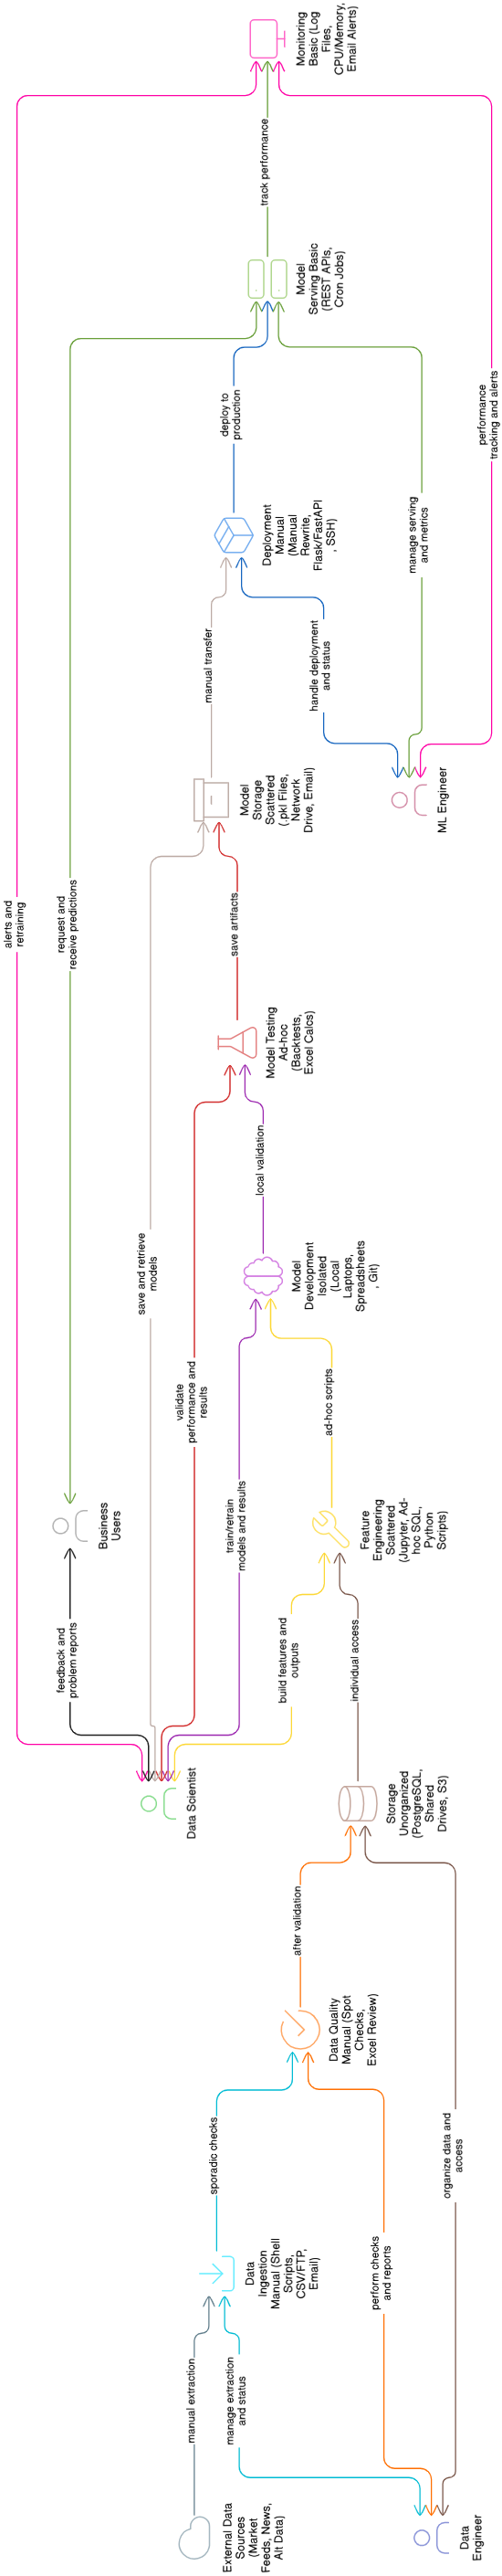
\includegraphics[width=0.32\textwidth]{figures/Fragment_General_Arch.png}
\caption{Arsitektur Terfragmentasi Saat Ini (General)}
\label{fig:general_fragmented_flow}
\end{figure}

Arsitektur pada Gambar~\ref{fig:general_fragmented_flow} mewakili pola Level 0/1 MLOps sebagaimana dibahas \textcite{kreuzberger2023mlops}. Untuk menautkan gejala arsitektural dengan pengalaman peran di lapangan, pola umum tersebut diurai menjadi alur berbasis \textit{persona} pada Gambar~\ref{fig:data_engineer_fragmented_flow} hingga Gambar~\ref{fig:business_user_fragmented_flow}. Penguraian ini memperlihatkan bahwa fragmentasi yang sama muncul dengan bentuk berbeda di tiap peran, tetapi menghasilkan konsekuensi operasional yang saling berkaitan. Dengan pendekatan ini, hubungan antara masalah di tingkat sistem dan hambatan sehari-hari \textit{Data Engineer}, \textit{Data Scientist}, \textit{ML Engineer}, dan \textit{Business Users} dapat diamati secara lebih konkret, dan hal tersebut menjadi dasar perancangan arsitektur pada subseksi berikutnya.

Gambar~\ref{fig:data_engineer_fragmented_flow} memperlihatkan silo di bagian hulu. \textit{Data Engineer} (DE) bertanggung jawab atas \textit{data ingestion} dan pemeriksaan kualitas secara manual sebelum menempatkan data pada \textit{Storage} (Unorganized). Setelah data tersimpan, DE memiliki visibilitas terbatas terhadap bagaimana data digunakan, model apa yang mengonsumsi data tersebut, dan siapa saja pemakai hilirnya. Ketidakjelasan ini menyulitkan penerapan tata kelola menyeluruh dari hulu ke hilir dan membuat upaya \textit{data stewardship} berhenti pada aspek teknis semata. Dalam jangka panjang, kondisi tersebut mendorong munculnya \textit{feature engineering} berulang dan tidak terkoordinasi pada lapisan berikutnya.

\begin{figure}[H]
\centering
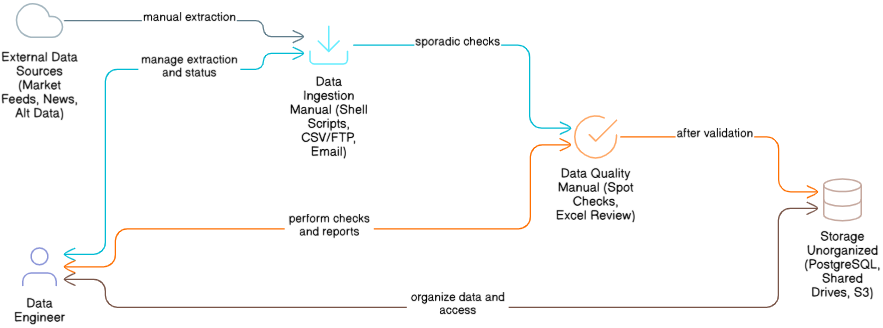
\includegraphics[width=\textwidth]{figures/Fragment_DatEng_Arch.png}
\caption{Arsitektur Terfragmentasi Saat Ini (Data Engineer)}
\label{fig:data_engineer_fragmented_flow}
\end{figure}

Gambar~\ref{fig:data_scientist_fragmented_flow} menggambarkan silo pada tahap pengembangan model. \textit{Data Scientist} (DS) mengambil data dari \textit{storage} yang tersebar, kemudian membangun fitur dan model di lingkungan terpisah seperti \textit{local laptop} atau \textit{notebook} yang berdiri sendiri. Lingkungan ini biasanya berada di luar \textit{pipeline} produksi, sehingga pelacakan eksperimen dan pengelolaan artefak sulit diintegrasikan dengan sistem operasional. Akibatnya, hasil eksperimen yang baik sering hanya terdokumentasi pada level individu, dan transisi dari eksperimen ke produksi kembali memerlukan kerja ulang dari nol. Pola ini membuat siklus iterasi menjadi lambat dan meningkatkan risiko hilangnya konteks teknis maupun bisnis yang melekat pada suatu model.

\begin{figure}[H]
\centering
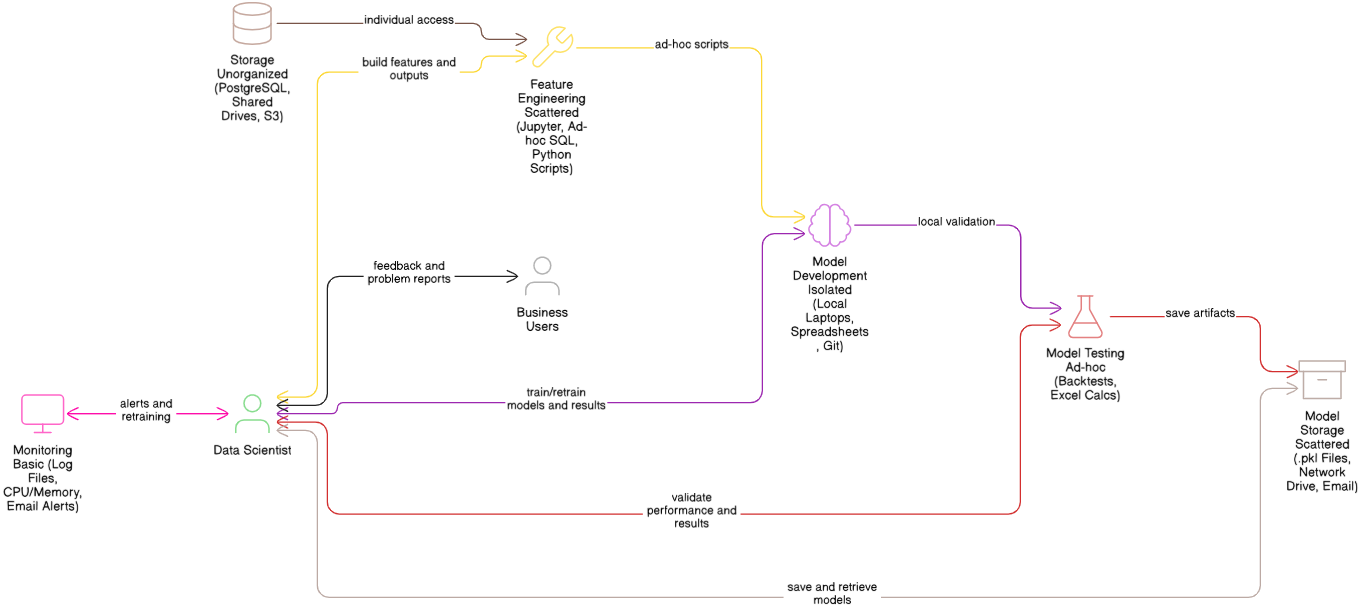
\includegraphics[width=\textwidth]{figures/Fragment_DatSci_Arch.png}
\caption{Arsitektur Terfragmentasi Saat Ini (Data Scientist)}
\label{fig:data_scientist_fragmented_flow}
\end{figure}

Dua konsekuensi utama dari alur tersebut adalah \textit{training--serving skew} dan \textit{monitoring} yang reaktif. \textit{Training--serving skew} muncul karena logika fitur yang dibangun DS pada tahap pelatihan tidak identik dengan logika \textit{inference} yang kemudian diimplementasikan \textit{ML Engineer} (MLE), sehingga perilaku model di pelatihan dan produksi berbeda \autocite{polyzotis2018data}. \textit{Monitoring} menjadi reaktif karena DS biasanya baru mengetahui kondisi model di produksi dari \textit{problem reports} yang disampaikan \textit{Business Users} (BU), bukan dari \textit{dashboard} teknis. Pola ini menyebabkan degradasi model baru terdeteksi setelah dampaknya terhadap bisnis cukup besar, dan siklus perbaikan menjadi panjang karena penelusuran kembali ke data dan konfigurasi awal tidak didukung oleh sistem terintegrasi.

Gambar~\ref{fig:ml_engineer_fragmented_flow} memperlihatkan silo di sisi MLE. MLE mengambil artefak model dari \textit{Model Storage} yang lokasinya tersebar, lalu melakukan \textit{manual rewrite} dari kode eksperimen menjadi layanan produksi berbasis Flask/FastAPI atau kerangka serupa. Proses ini biasanya melibatkan \textit{refactoring} besar dan penambahan lapisan \textit{logging}, \textit{monitoring}, dan keamanan. Pekerjaan tersebut menyita banyak waktu dan berisiko tinggi menimbulkan \textit{bug}, sehingga \textit{lead time} dari eksperimen ke produksi menjadi panjang. Dalam jangka panjang, pola ini justru menambah \textit{technical debt} baru yang harus dikelola \autocite{paleyes2022challenges} dan menghambat kemampuan organisasi untuk bereksperimen dengan model baru secara cepat.

\begin{figure}[H]
\centering
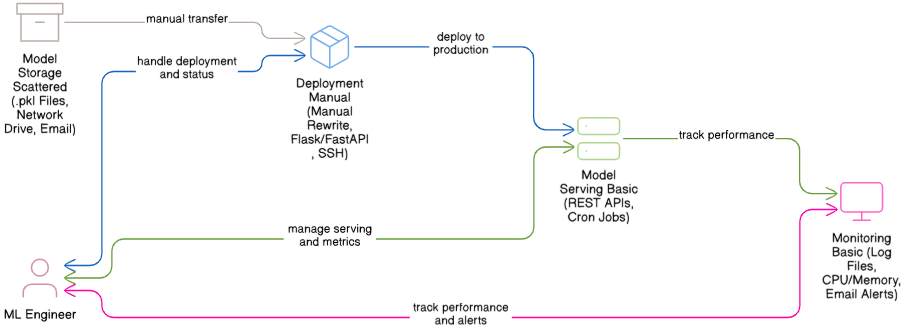
\includegraphics[width=\textwidth]{figures/Fragment_MLEng_Arch.png}
\caption{Arsitektur Terfragmentasi Saat Ini (ML Engineer)}
\label{fig:ml_engineer_fragmented_flow}
\end{figure}

Gambar~\ref{fig:business_user_fragmented_flow} menempatkan \textit{Business Users} (BU) sebagai pihak di tepi sistem yang perannya cenderung pasif. BU hanya dapat mengajukan permintaan prediksi, menerima hasil, lalu melaporkan masalah ketika keluaran dianggap tidak memuaskan atau berdampak negatif. BU umumnya tidak memiliki akses \textit{self-service} ke data atau model serta tidak memiliki visibilitas terhadap status sistem. Situasi ini memperkuat paradigma reaktif dan menyulitkan organisasi membangun budaya pengambilan keputusan berbasis data yang konsisten. \textit{Feedback loop} dari bisnis ke tim teknis akhirnya berjalan lambat dan tidak terstruktur.

\begin{figure}[H]
\centering
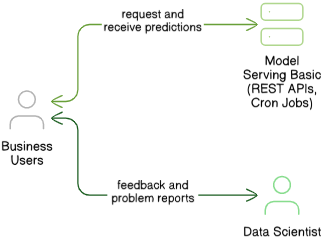
\includegraphics[width=0.5\textwidth]{figures/Fragment_BusUs_Arch.png}
\caption{Arsitektur Terfragmentasi Saat Ini (Business Users)}
\label{fig:business_user_fragmented_flow}
\end{figure}

\noindent Karakteristik masalah yang berulang pada pola terfragmentasi dapat dirangkum sebagai berikut:

\vspace{0.5em}
\begin{enumerate}
    \item \textbf{\textit{Heterogeneous Compute Infrastructure}}  

    Infrastruktur masih banyak bergantung pada \textit{provisioning} manual, waktu tunggu \textit{scaling} yang panjang, dan tingkat standardisasi konfigurasi yang rendah. Perbedaan konfigurasi antartim dan antarlingkungan membuat portabilitas dan reproduksibilitas sulit dicapai. Arsitektur usulan merespons kondisi ini dengan pendekatan \textit{vertical scaling} untuk \textit{batch}, \textit{horizontal scaling} untuk \textit{stream}, dan kombinasi keduanya untuk \textit{real-time inference}, lalu mengevaluasi pendekatan tersebut menggunakan kerangka skalabilitas \textcite{jogalekar2000evaluating}.

    \vspace{0.5em}

    \item \textbf{Fragmentasi \textit{Feature Engineering}}  

    Logika fitur tersebar di berbagai \textit{notebook} dan skrip, sehingga duplikasi dan inkonsistensi definisi fitur menjadi tinggi. Ketiadaan repositori terpusat yang mencatat definisi, dependensi, dan pemilik fitur membuat \textit{troubleshooting} dan \textit{impact analysis} sulit dilakukan. Fragmentasi ini juga menghambat \textit{reuse} fitur antartim karena tidak ada titik referensi bersama yang disepakati.

    \vspace{0.5em}

    \item \textbf{Lingkungan Pengembangan Terisolasi}  

    DS mengembangkan model di lingkungan lokal yang tidak terhubung dengan sistem produksi, sehingga praktik \textit{experiment tracking} dan pengelolaan artefak sering bersifat \textit{ad hoc}. Pengetahuan yang dihasilkan sulit ditransfer ke tim lain dan sulit diulang kembali. Perbedaan lingkungan yang lebar memaksa tim melakukan \textit{refactoring} besar saat memindahkan model ke produksi.

    \vspace{0.5em}

    \item \textbf{Proses \textit{Deployment} Manual}  

    \textit{Deployment} model masih mengandalkan \textit{manual rewrite} dari kode eksperimen ke layanan produksi, sehingga risiko \textit{bug} meningkat dan praktik \textit{continuous delivery} sulit diterapkan. \textit{Lead time} dari perubahan kecil ke \textit{deployment} produksi menjadi tidak terprediksi \autocite{paleyes2022challenges}. Kondisi ini bertentangan dengan praktik modern pengiriman perangkat lunak yang mendorong rilis cepat dan sering.

    \vspace{0.5em}

    \item \textbf{Paradigma \textit{Monitoring} Reaktif}  

    \textit{Monitoring} masih berfokus pada metrik infrastruktur, sementara metrik ML spesifik jarang diinstrumentasi. \textit{Drift} jarang dipantau secara sistematis meskipun \textcite{jourdan2023handling} menunjukkan bahwa \textit{retraining} yang dipicu deteksi \textit{drift} dapat meningkatkan akurasi dari 0{,}5400 menjadi 0{,}7010. Tanpa \textit{monitoring} proaktif, sistem cenderung merespons masalah setelah dampak bisnis terjadi.

    \vspace{0.5em}

    \item \textbf{Kesenjangan \textit{Governance}}  

    \textit{Lineage} dan \textit{audit trail} jarang dilacak otomatis, sehingga pemenuhan \textit{compliance} menjadi sulit dan beban administratif saat audit meningkat. Dokumentasi aset data dan model tersebar serta tidak selalu sinkron dengan keadaan produksi. Dalam lingkungan yang diawasi regulator, kondisi ini meningkatkan risiko ketidaksesuaian dan sanksi.

    \vspace{0.5em}
\end{enumerate}

Permasalahan lain yang penting adalah \textit{training--serving skew} dan validitas temporal pada data \textit{time-series}. Skew muncul ketika logika fitur pada tahap pelatihan tidak persis sama dengan logika \textit{inference} di produksi, sehingga model gagal mempertahankan performa setelah di-\textit{deploy} \autocite{polyzotis2018data}. Tanpa \textit{feature store} terpusat, perbedaan ini menjadi masalah laten yang sulit dideteksi dan mudah terulang. Pada data perdagangan, kebocoran data temporal juga mengancam validitas model dan membuat hasil \textit{backtesting} terlalu optimistis \autocite{polyzotis2018data,wang2021leakage}. Implementasi \textit{point-in-time correct join} secara manual di berbagai lingkungan terpisah sangat rentan kesalahan, sehingga risiko kebocoran mudah berulang di banyak \textit{pipeline} tanpa terdeteksi.

\subsection{Arsitektur Sistem yang Diusulkan: Platform Terintegrasi}

Arsitektur yang diusulkan mengubah pola \textit{loosely coupled tools} menjadi platform DataOps--MLOps terintegrasi yang menopang siklus hidup ML secara menyeluruh. Platform ini menyatukan \textit{workflow} utama, meningkatkan otomasi, dan menambahkan lapisan \textit{governance} yang eksplisit sehingga hambatan pada arsitektur eksisting dapat diatasi secara sistematis. Desain mengadopsi prinsip \textit{microservices} dengan \textit{API Gateway} \autocite{fowler2014microservices,newman2015building}, infrastruktur deklaratif, GitOps, dan pendekatan \textit{observability-driven}. Lapisan keamanan dibangun berlapis dengan JWT, OAuth 2.0, dan mTLS yang dipadukan dengan \textit{centralized identity} dan \textit{access orchestration}. Dalam konfigurasi ini, \textit{identity provider} seperti Frontier menangani otentikasi, sementara \textit{access workflow engine} seperti Guardian mengelola permintaan akses terhadap aset data secara terdokumentasi dan dapat diaudit, sejalan dengan pola RBAC dan prinsip \textit{least privilege}.

Gambar~\ref{fig:general_integrated_flow} memperlihatkan pergeseran alur dari pola linear yang sarat proses manual menjadi pola \textit{hub-and-spoke} dengan tiga pilar utama. Tiga pilar tersebut adalah GitOps (ArgoCD) sebagai sumber kebenaran konfigurasi, \textit{Governance} (DataHub) sebagai pusat metadata dan \textit{lineage}, serta \textit{Observability} (Prometheus, Grafana, dan komponen terkait) sebagai landasan pemantauan \autocite{googlecloud2024mlops,kreuzberger2023mlops,cncf2024observability}. Lapisan keamanan dan akses yang melibatkan Frontier, Guardian, mekanisme \textit{secrets management}, dan \textit{API Gateway} berjalan melintang di atas ketiga pilar tersebut dan melindungi seluruh alur. Dengan struktur ini, setiap perubahan, insiden, dan keputusan operasional selalu dapat dirujuk kembali ke informasi yang konsisten dan tersimpan di satu tempat.

\begin{figure}[H]
\centering
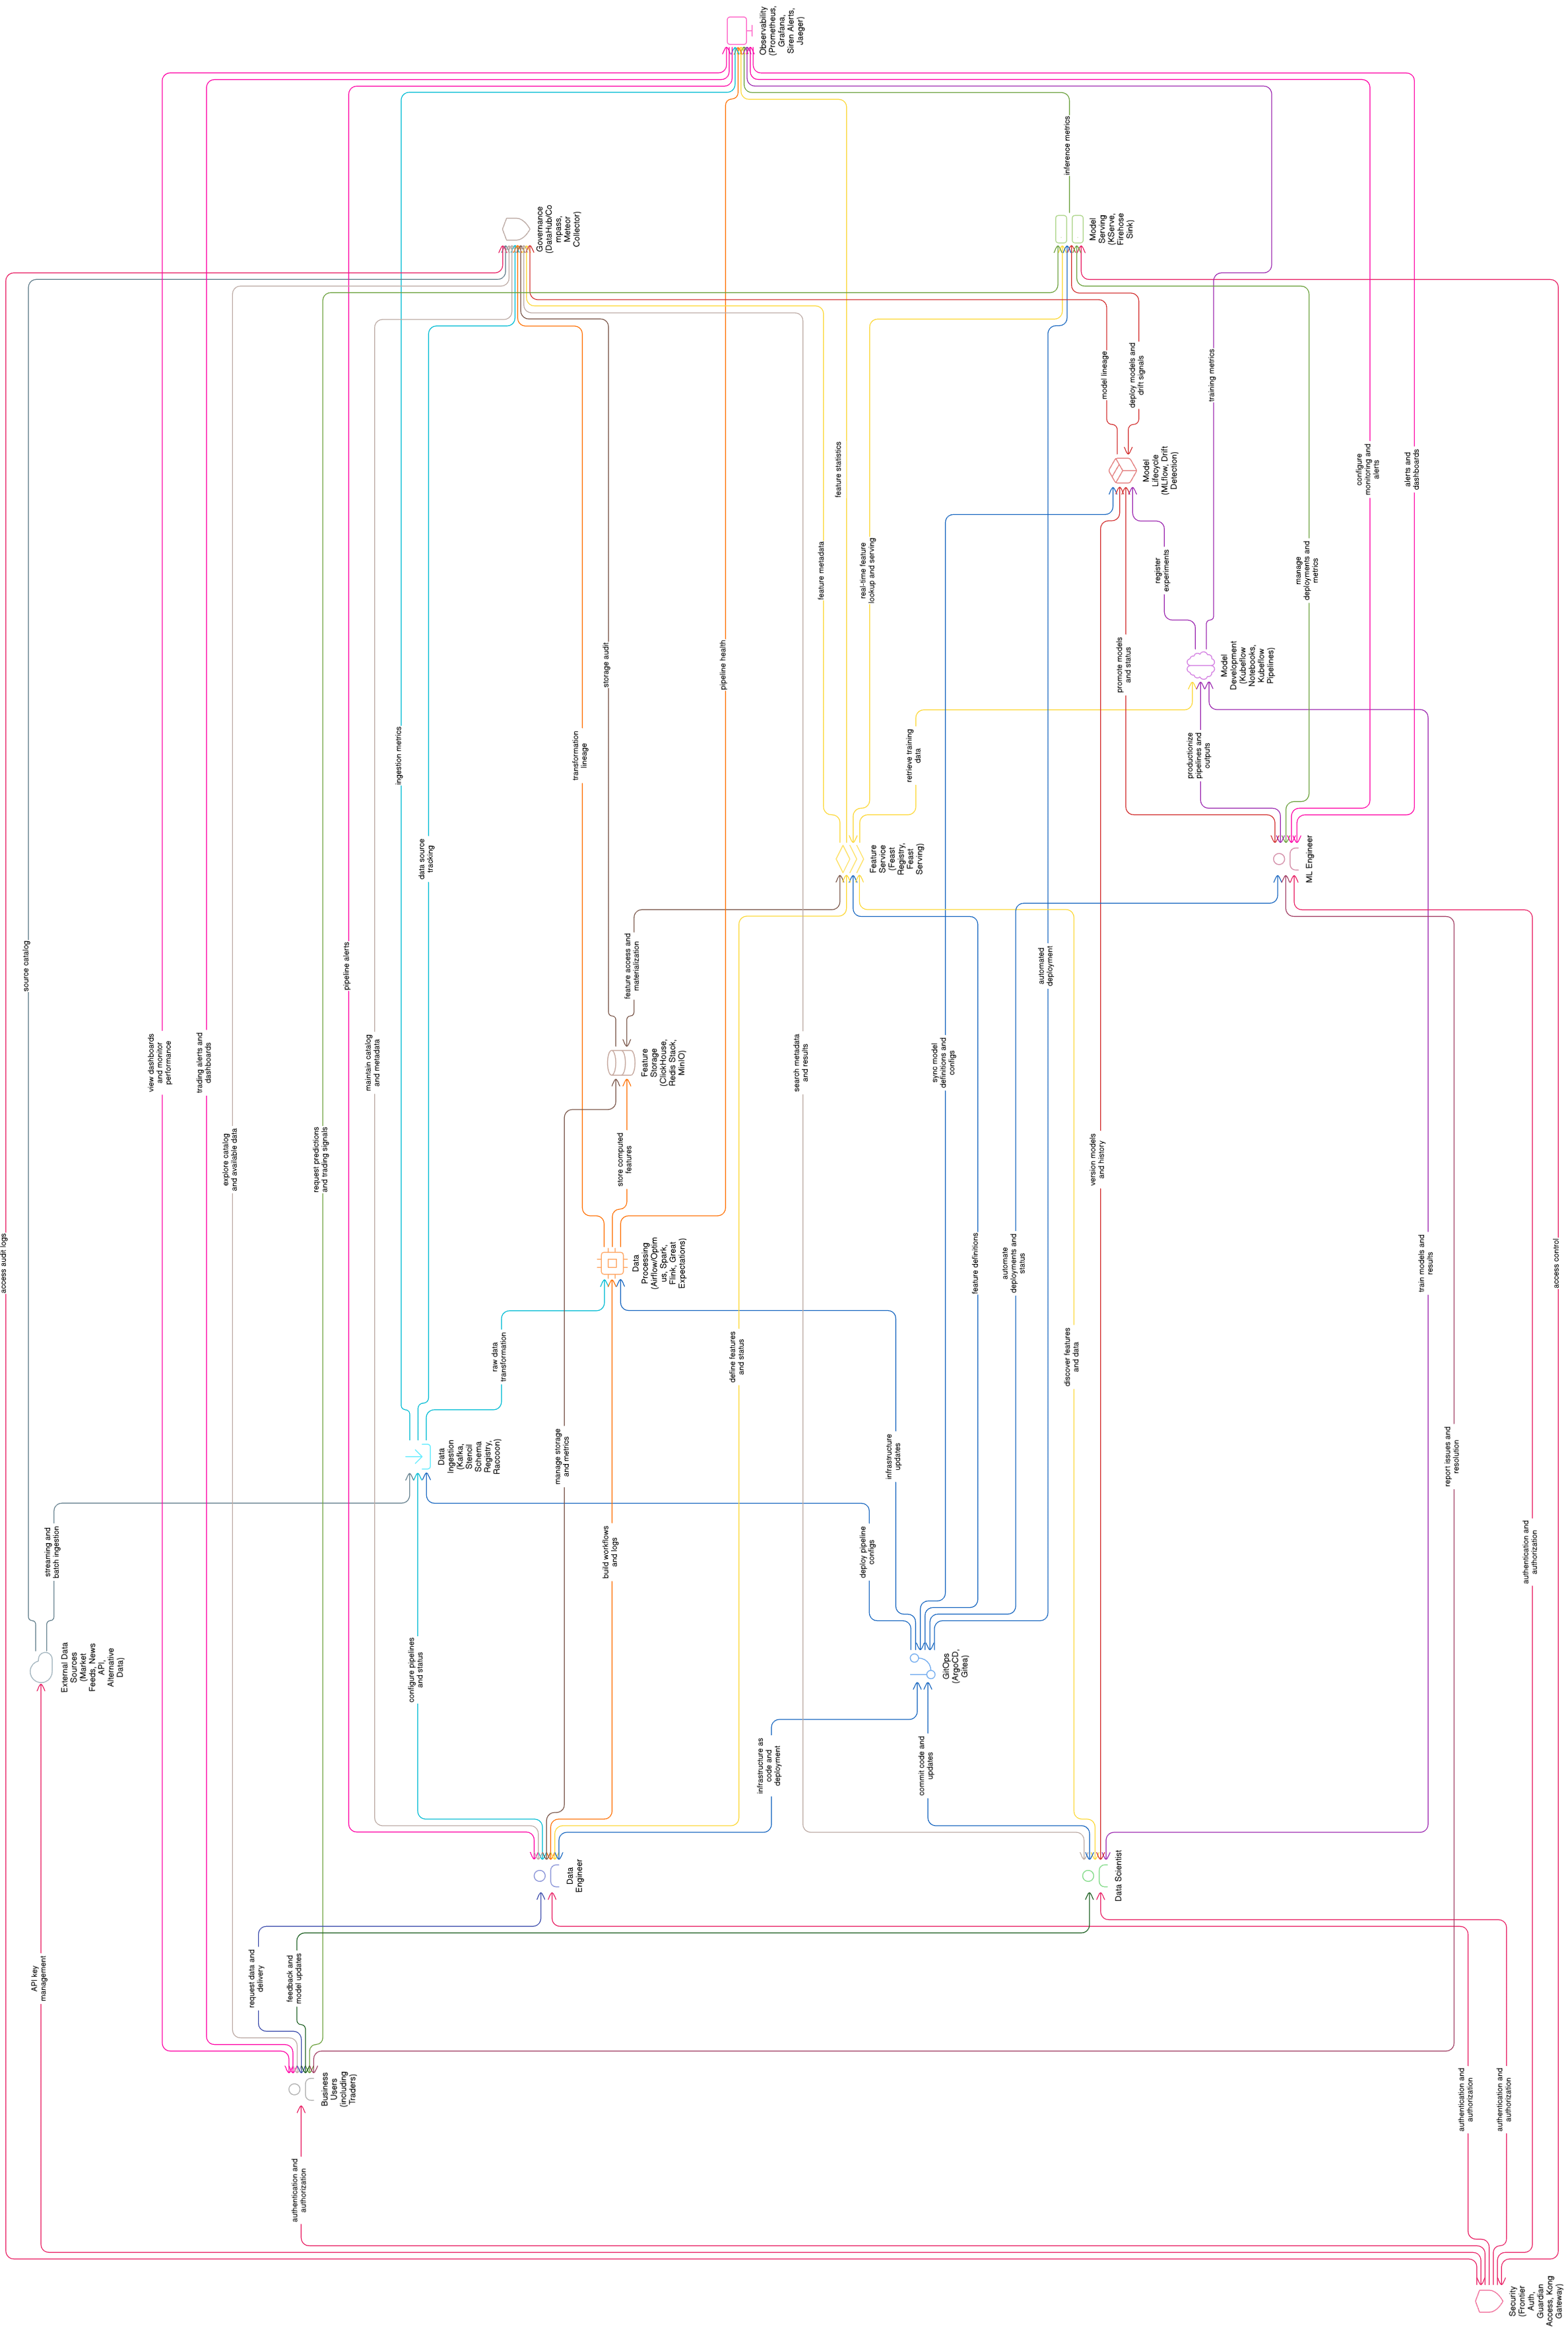
\includegraphics[width=\textwidth]{figures/Integrate_General_Arch.png}
\caption{Arsitektur Terintegrasi yang Diusulkan (General)}
\label{fig:general_integrated_flow}
\end{figure}

Arsitektur baru dirancang untuk mengurangi silo di setiap \textit{persona}. Semua komponen fungsional dan peran dihubungkan melalui tiga pilar sentral, sejalan dengan Level 2 pada \textit{Google Cloud MLOps framework} \autocite{googlecloud2024mlops,kreuzberger2023mlops}. Dengan penyusunan seperti ini, perubahan di satu area dapat dikendalikan dan diaudit secara menyeluruh karena selalu terekam pada pilar GitOps, Governance, dan Observability. Konsekuensinya, reliabilitas sistem dan kualitas tata kelola meningkat, sementara friksi antartim menurun dan \textit{feedback loop} bisnis–teknis menjadi lebih pendek.

Gambar~\ref{fig:data_engineer_integrated_flow} menunjukkan bahwa DE tidak lagi mengelola \textit{pipeline} secara manual per komponen, tetapi mengoperasikan \textit{pipeline} otomatis yang menghubungkan \textit{Data Ingestion} (Kafka) dengan \textit{Data Processing} (Airflow, Spark, Flink). Pada sisi tepi, \textit{event collector} seperti Raccoon menerima \textit{event} ber-throughput tinggi dari aplikasi perdagangan dan meneruskannya ke Kafka, sementara \textit{schema registry} seperti Stencil menjaga konsistensi \textit{schema} dan evolusinya. Definisi \textit{job} dan jadwal disimpan di Git dan disinkronkan menggunakan GitOps, aset dan \textit{lineage}-nya tercatat di DataHub, dan reliabilitas \textit{pipeline} dipantau melalui lapisan \textit{observability}. Dengan pola ini, keterkaitan hulu–hilir data menjadi transparan dan dapat dikelola secara terpusat.

\begin{figure}[H]
\centering
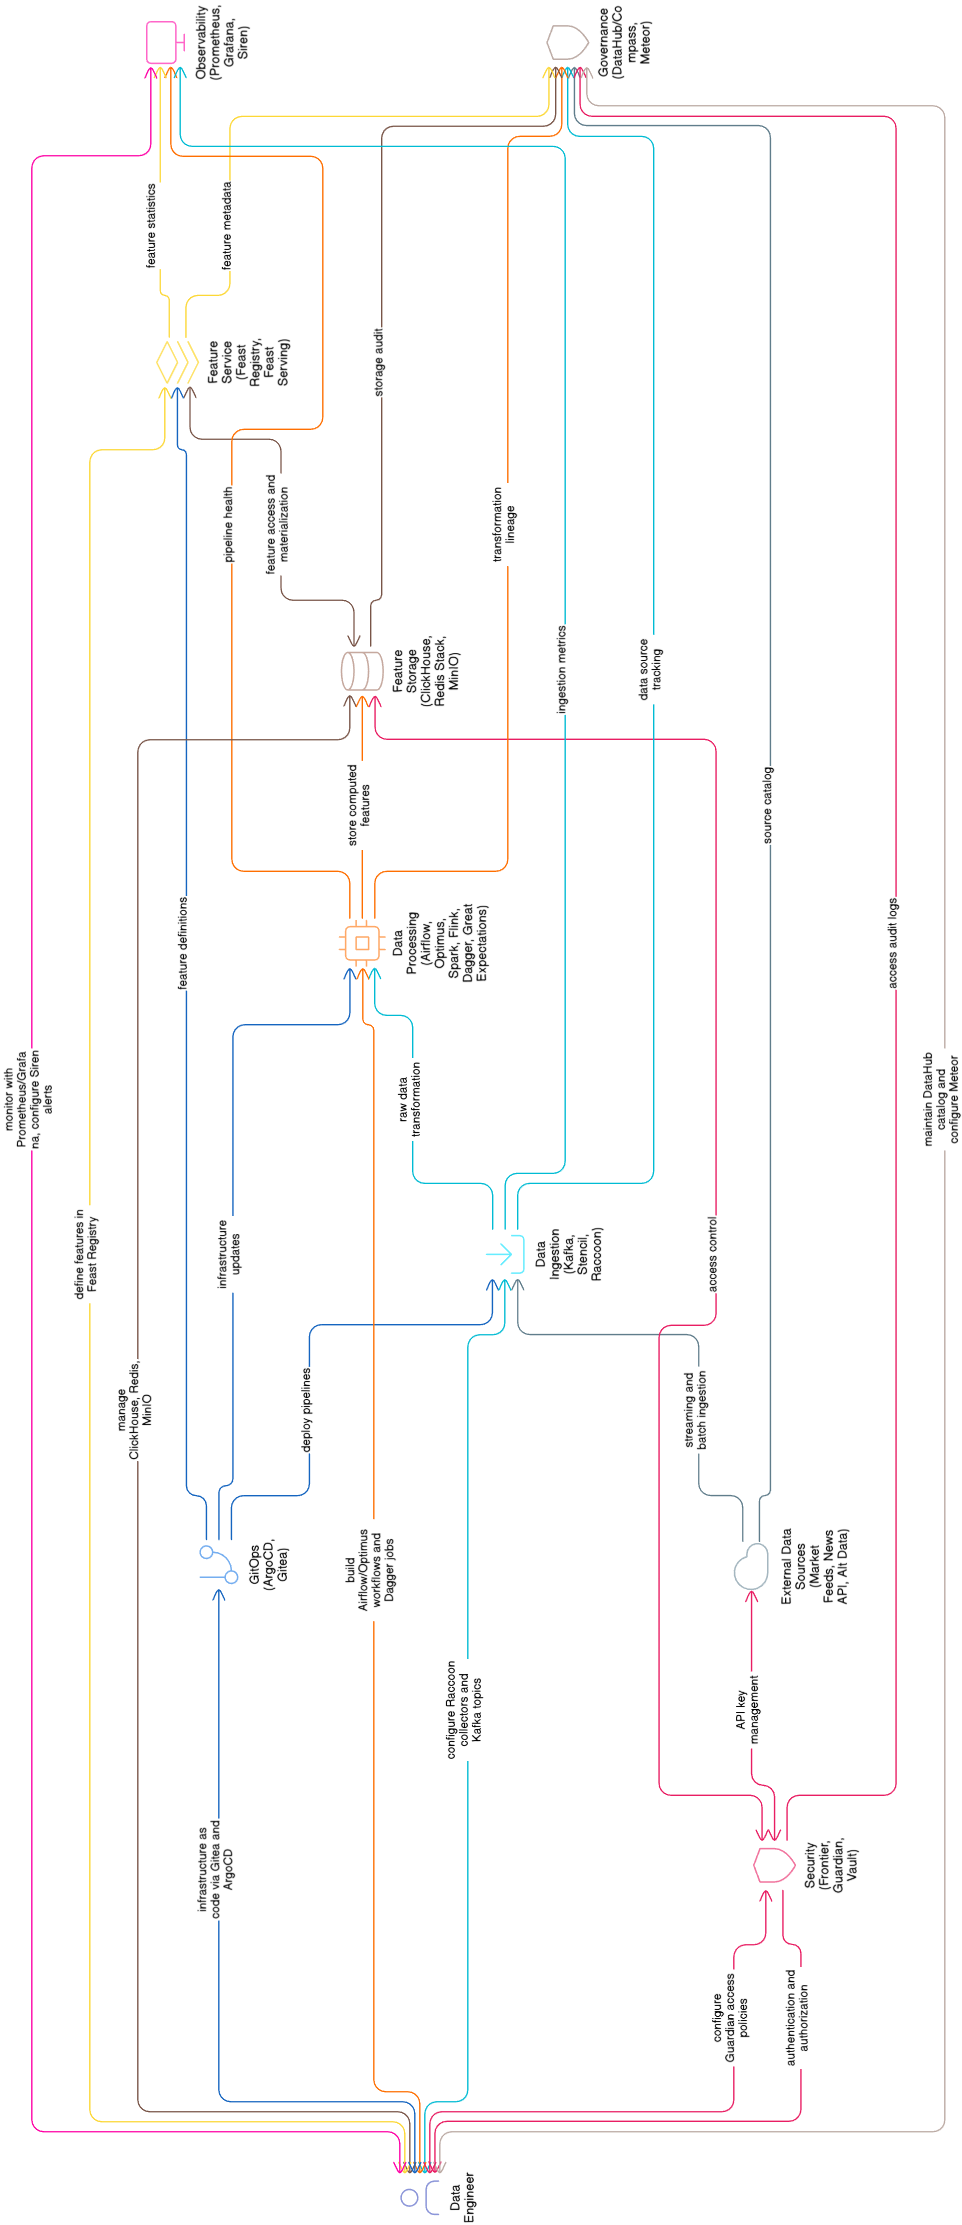
\includegraphics[width=0.7\textwidth]{figures/Integrate_DatEng_Arch.png}
\caption{Arsitektur Terintegrasi yang Diusulkan (Data Engineer)}
\label{fig:data_engineer_integrated_flow}
\end{figure}

Gambar~\ref{fig:data_scientist_integrated_flow} memperlihatkan bahwa DS mengakses fitur melalui \textit{Feature Service} (Feast) yang menyediakan definisi konsisten untuk pelatihan dan \textit{serving}. Eksperimen dijalankan pada Kubeflow Notebooks atau Kubeflow Pipelines yang berada di klaster yang sama dengan produksi sehingga perbedaan lingkungan dapat diminimalkan. Aset data, fitur, dan model dapat ditelusuri melalui DataHub, sehingga konteks teknis dan bisnis tidak terputus ketika model berpindah tahap. \textit{Experiment tracking} dilakukan dengan MLflow, dan akses ke dataset serta fitur dikelola oleh Guardian agar tetap selaras dengan kebijakan akses organisasi.

\begin{figure}[H]
\centering
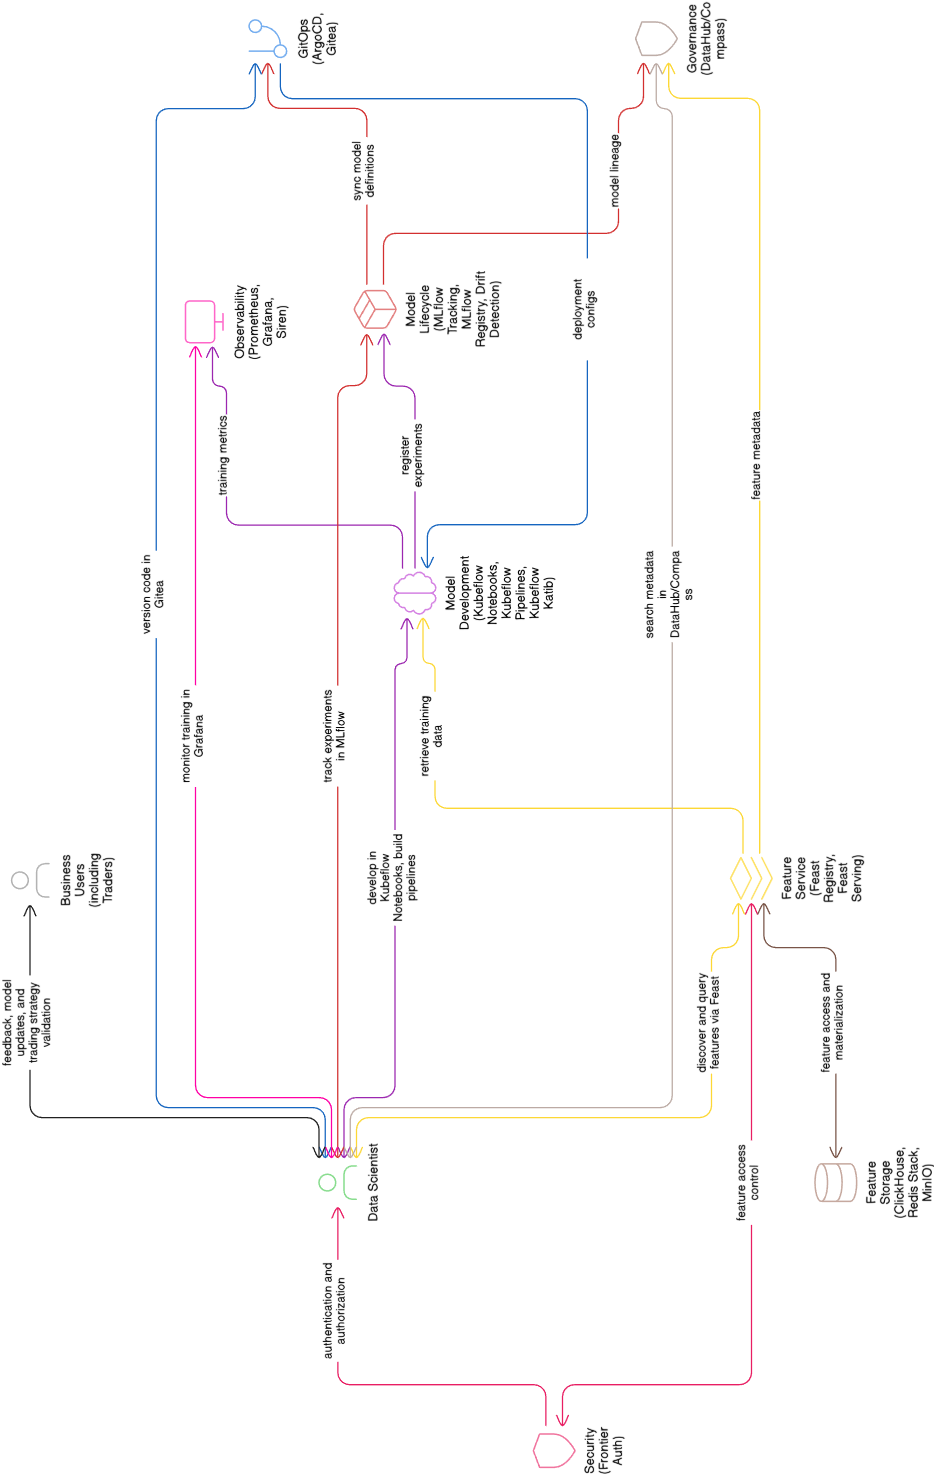
\includegraphics[width=\textwidth]{figures/Integrate_DatSci_Arch.png}
\caption{Arsitektur Terintegrasi yang Diusulkan (Data Scientist)}
\label{fig:data_scientist_integrated_flow}
\end{figure}

Gambar~\ref{fig:ml_engineer_integrated_flow} menunjukkan bahwa MLE tidak lagi melakukan \textit{rewrite} manual dari model ke layanan produksi. MLE mempromosikan model melalui MLflow \textit{registry}, yang kemudian memicu pembaruan konfigurasi di Git untuk sumber daya KServe. ArgoCD menyinkronkan konfigurasi tersebut ke klaster dan menyiapkan \textit{deployment} secara deklaratif, sehingga kesalahan manusia berkurang dan proses \textit{deployment} menjadi lebih dapat diprediksi. Metrik kinerja dan \textit{drift} dimonitor lewat \textit{observability stack}, sementara \textit{sink service} seperti Firehose digunakan untuk menyalurkan log prediksi dan \textit{feedback} ke data store analitik agar siklus \textit{monitoring} dan \textit{retraining} dapat diotomasi.

\begin{figure}[H]
\centering
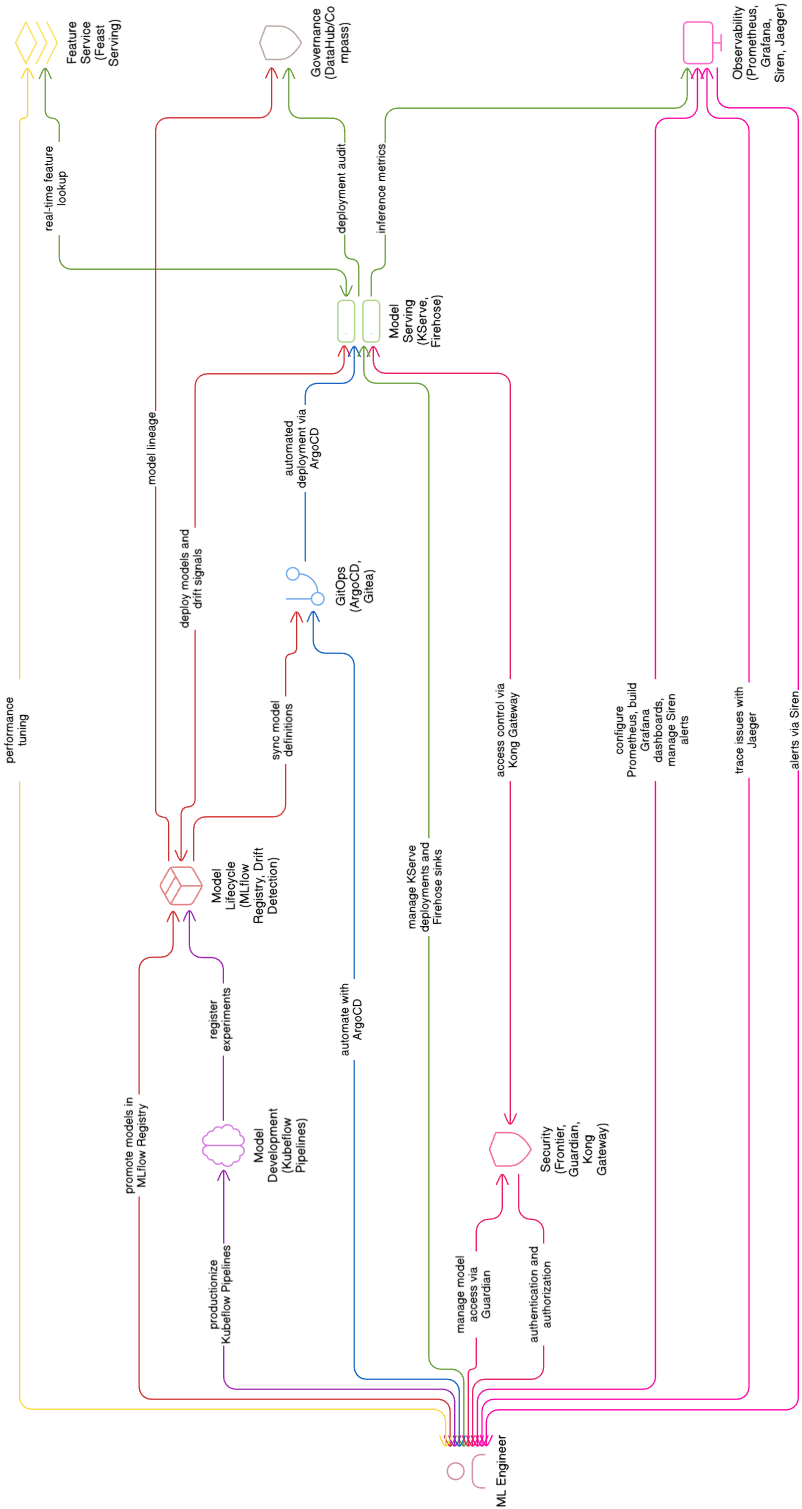
\includegraphics[width=0.85\textwidth]{figures/Integrate_MLEng_Arch.png}
\caption{Arsitektur Terintegrasi yang Diusulkan (ML Engineer)}
\label{fig:ml_engineer_integrated_flow}
\end{figure}

Gambar~\ref{fig:business_user_integrated_flow} menunjukkan bahwa BU diposisikan sebagai bagian yang lebih aktif di dalam platform, bukan sekadar penerima hasil. BU dapat mengakses \textit{dashboard} KPI dan metrik model secara \textit{real-time} untuk memantau kinerja strategi perdagangan. Selain itu, BU dapat menelusuri data dan model di DataHub maupun katalog ringan seperti Compass untuk memahami konteks prediksi yang digunakan. Pola ini memperpendek \textit{feedback loop} antara perspektif teknis dan bisnis dan memungkinkan diskusi yang lebih berbasis data, sehingga keputusan bisnis dapat dikaitkan langsung dengan kondisi aktual sistem.

\begin{figure}[H]
\centering
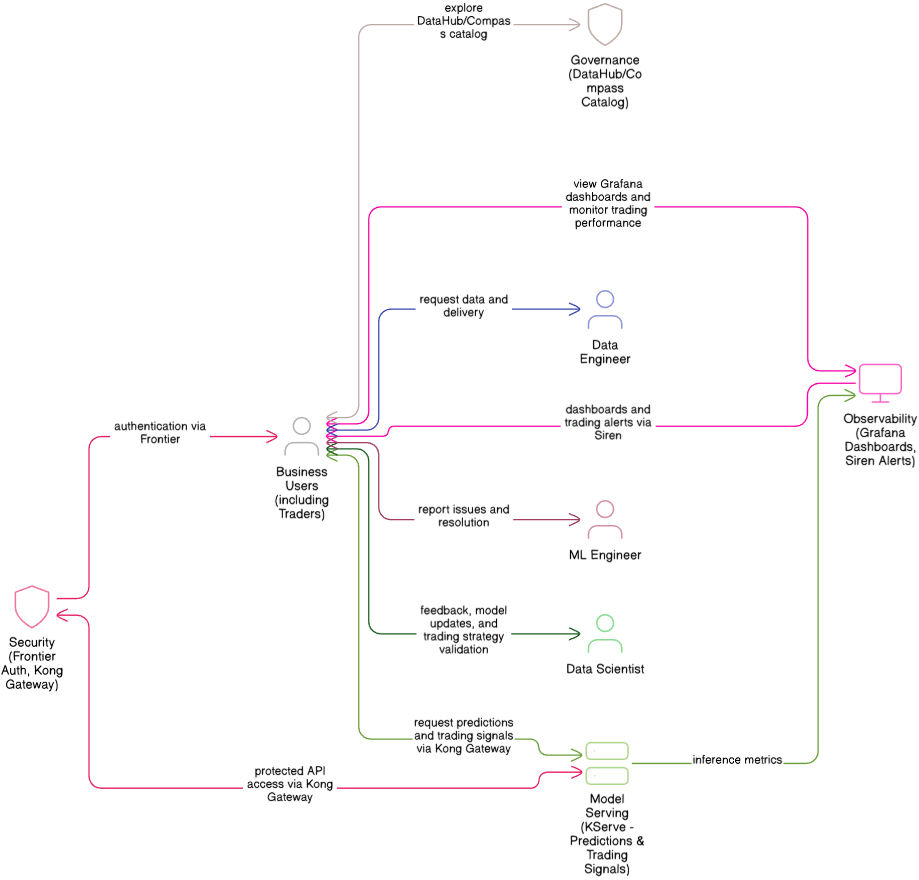
\includegraphics[width=\textwidth]{figures/Integrate_BusUs_Arch.png}
\caption{Arsitektur Terintegrasi yang Diusulkan (Business Users)}
\label{fig:business_user_integrated_flow}
\end{figure}

Kubernetes dipilih sebagai lapisan orkestrasi utama karena tingkat adopsi yang luas, dukungan yang baik terhadap \textit{workload} ML, portabilitas lintas \textit{cloud}, dan kemampuan mereproduksi lingkungan berbasis kontainer. Komponen fungsional disusun ke dalam beberapa lapisan arsitektur untuk memisahkan \textit{concerns} dan memungkinkan setiap lapisan diskalakan secara independen \autocite{kleppmann2017ddia,marz2015lambda,stopford2018designing}. Penyusunan berlapis ini memudahkan pemetaan tanggung jawab dan memberikan fleksibilitas ketika organisasi ingin menambah atau mengganti komponen di masa mendatang. Rincian kontribusi setiap lapisan terhadap kebutuhan sistem dibahas lebih lanjut pada bagian \textit{Desain Detail Lapisan Arsitektur} di bab ini sebagai dasar implementasi.

GitOps digunakan untuk memastikan konfigurasi \textit{deployment} dan infrastruktur dikelola sebagai kode di Git, dengan ArgoCD sebagai komponen yang menyinkronkan keadaan klaster dengan isi repositori. Pola ini menyediakan \textit{audit trail}, memudahkan \textit{rollback}, dan meningkatkan reproduksibilitas ketika terjadi insiden atau percobaan konfigurasi baru. Dengan pendekatan ini, perubahan terhadap komponen Raystack maupun komponen lain dikelola melalui mekanisme kontrol versi yang sama di seluruh lapisan. Siklus perubahan konfigurasi dan \textit{deployment} menjadi konsisten, sehingga risiko perubahan tak terpantau dapat dikurangi.

\subsection{Analisis Perbedaan Kunci}

Perbandingan antara arsitektur eksisting dan arsitektur terintegrasi menunjukkan pergeseran dari Level 0/1 menuju Level 2 MLOps \textcite{kreuzberger2023mlops}. Pergeseran ini menyentuh sisi teknologi, pola kerja lintas tim, dan cara organisasi mengelola risiko operasional. Tabel~\ref{tab:architecture_comparison} merangkum perbedaan utama dari sisi teknis, konfigurasi yang diusulkan, dan manfaat yang ditargetkan. Penyajian dalam bentuk tabel memudahkan pembaca melihat hubungan langsung antara keputusan desain dan dampak operasional tanpa perlu menelusuri seluruh penjelasan naratif.

{
\footnotesize
\begin{longtable}{|m{2cm}|m{2.5cm}|m{2.5cm}|m{3cm}|m{2cm}|}
\caption{\raggedright Perbandingan Detail Arsitektur Saat Ini dengan yang Diusulkan}
\label{tab:architecture_comparison} \\
\hline
\multicolumn{1}{|>{\centering\arraybackslash}m{2cm}|}{\textbf{Aspek}} &
\multicolumn{1}{>{\centering\arraybackslash}m{2.5cm}|}{\textbf{Arsitektur Saat Ini}} &
\multicolumn{1}{>{\centering\arraybackslash}m{2.5cm}|}{\textbf{Arsitektur Diusulkan}} &
\multicolumn{1}{>{\centering\arraybackslash}m{3cm}|}{\textbf{Keuntungan Terukur}} &
\multicolumn{1}{>{\centering\arraybackslash}m{2cm}|}{\textbf{Referensi}} \\
\hline
\endfirsthead
\hline
\multicolumn{1}{|>{\centering\arraybackslash}m{2cm}|}{\textbf{Aspek}} &
\multicolumn{1}{>{\centering\arraybackslash}m{2.5cm}|}{\textbf{Arsitektur Saat Ini}} &
\multicolumn{1}{>{\centering\arraybackslash}m{2.5cm}|}{\textbf{Arsitektur Diusulkan}} &
\multicolumn{1}{>{\centering\arraybackslash}m{3cm}|}{\textbf{Keuntungan Terukur}} &
\multicolumn{1}{>{\centering\arraybackslash}m{2cm}|}{\textbf{Referensi}} \\
\hline
\endhead
\hline
\endfoot
\hline
\endlastfoot

Orkestrasi &
\textit{Compute} heterogen dengan \textit{provisioning} manual, waktu tunggu \textit{scaling} panjang, dan tingkat standardisasi rendah. &
Platform Kubernetes terpadu dengan manajemen deklaratif dan alokasi sumber daya otomatis, sejalan dengan komponen arsitektur MLOps yang diidentifikasi \textcite{kreuzberger2023mlops}. GitOps dengan ArgoCD memastikan perubahan infrastruktur dan aplikasi (termasuk komponen Raystack) mengikuti \textit{single source of truth} di Git. &
Studi yang dirangkum \textcite{lakka2025kubernetes} menunjukkan bahwa organisasi \textit{high-performing} yang menerapkan praktik DevOps berbasis Kubernetes dapat meningkatkan \textit{deployment frequency} hingga 973$\times$ dan memperbaiki MTTR hingga 6570$\times$; arsitektur yang diusulkan menargetkan karakteristik performa yang serupa. &
\autocite{kreuzberger2023mlops,lakka2025kubernetes} \\
\hline
Manajemen Fitur &
Logika fitur tersebar di \textit{notebook} dan skrip dengan duplikasi tinggi dan banyak fungsi yang saling tumpang tindih. &
Feast dengan \textit{feature registry} terpusat, \textit{dual serving} \textit{offline/online}, serta dukungan \textit{point-in-time correctness}. &
Duplikasi fitur dapat ditekan, \textit{training--serving skew} berkurang melalui pemisahan \textit{offline/online} dan \textit{point-in-time retrieval}, dan \textit{feature reuse} berpotensi meningkat signifikan. &
\autocite{munappy2022data,polyzotis2018data} \\
\hline
\textit{Vector Embeddings} &
Fitur \textit{embedding} tidak didukung secara \textit{native} atau diimplementasikan secara kustom dengan latensi tinggi dan \textit{throughput} terbatas. &
Redis Stack dengan dukungan HNSW \textit{vector search} berlatensi rendah. &
\textcite{johnson2021billion} menunjukkan bahwa penggunaan FAISS pada GPU dapat memberikan percepatan hingga 8{,}5 kali pada dataset YFCC100M; desain ini memanfaatkan prinsip serupa untuk \textit{similarity search} berperforma tinggi. &
\autocite{johnson2021billion} \\
\hline
Validitas Temporal &
\textit{Point-in-time} \textit{join} dilakukan manual dan rentan kesalahan, sehingga banyak tim mengalami \textit{data leakage}. &
\textit{Point-in-time join} otomatis dari Feast dengan pola verifikasi yang lebih sistematis. &
Pendekatan ini mencegah kebocoran data temporal yang dapat menghasilkan estimasi performa \textit{backtest} yang terlalu optimistis dan tidak realistis di produksi. &
\autocite{polyzotis2018data} \\
\hline
Pemrosesan Data &
\textit{Batch} dan \textit{stream} diproses oleh \textit{pipeline} terpisah tanpa arsitektur yang koheren, sehingga hasil pemrosesan tidak konsisten. &
Spark sebagai mesin \textit{batch processing} dan Flink sebagai mesin \textit{stream processing} yang hasilnya dimaterialisasikan langsung ke \textit{Feature Store}. Optimus dan Dagger memfasilitasi definisi \textit{pipeline} berbasis konfigurasi sehingga pengembangan dan pengelolaan jadwal transformasi menjadi lebih sistematis. &
Waktu pengembangan \textit{pipeline} dapat menurun dan \textit{freshness} data meningkat berkat pemrosesan \textit{streaming} yang lebih efisien dan terintegrasi. &
\autocite{rodrigues2025architecture} \\
\hline
Pelatihan Model &
\textit{Workflow} pelatihan berbasis \textit{notebook} dengan \textit{tracking} eksperimen informal dan \textit{artifact} tidak terkelola. &
Kubeflow \textit{Pipelines} untuk orkestrasi pelatihan dan MLflow untuk \textit{tracking} eksperimen. &
Reprodusibilitas meningkat melalui kontainerisasi dan pengelolaan eksperimen terpusat, sementara siklus pengembangan \textit{pipeline} menjadi lebih terstruktur. &
\autocite{amershi2019software,pimentel2019notebooks} \\
\hline
\textit{Deployment} Model &
Proses \textit{deployment} manual dengan \textit{refactoring} besar dan sering terjadi \textit{bug} pasca-\textit{deploy}. &
KServe dengan \textit{InferenceService} deklaratif dan \textit{deployment} otomatis melalui GitOps. Firehose dapat digunakan untuk menyalurkan log \textit{inference} ke data store secara konsisten sebagai dasar \textit{monitoring} dan analitik lanjutan. &
Waktu \textit{deployment} berpotensi turun secara signifikan, dan insiden terkait kesalahan konfigurasi \textit{deployment} dapat dikurangi lewat otomasi. &
\autocite{paleyes2022challenges} \\
\hline
Pola \textit{Deployment} Lanjut &
Pola seperti \textit{canary release} jarang digunakan, organisasi umumnya mengandalkan \textit{binary switchover}. &
Dukungan \textit{canary release}, A/B \textit{testing}, dan \textit{automatic rollback} prediktif. &
\textit{Rollout} dapat dilakukan secara bertahap dan aman, sehingga MTTR menurun karena kegagalan dapat dibatasi pada \textit{canary traffic}. &
\autocite{shankar2022operationalizing} \\
\hline
Deteksi \textit{Drift} &
Deteksi \textit{drift} bersifat reaktif dengan jeda deteksi yang panjang terhadap isu penting dan perubahan gradual. &
\textit{Monitoring} proaktif dengan uji statistik, \textit{alert real-time}, dan penetapan ambang adaptif. &
Jeda deteksi \textit{drift} dapat dipersingkat sehingga \textit{retraining} dapat dijadwalkan lebih tepat waktu untuk menjaga kinerja model. &
\autocite{cespedes2024efficient,bayram2022concept} \\
\hline
\textit{Governance} \& \textit{Lineage} &
Dokumentasi dilakukan secara manual dan \textit{audit trail} sering tidak lengkap atau tersebar. &
DataHub dengan \textit{metadata ingestion} otomatis (dibantu Meteor) dan \textit{lineage} yang dapat ditelusuri dari \textit{source} hingga model; Compass dapat melengkapi sebagai katalog ringan untuk aset tertentu. &
Waktu persiapan audit dapat berkurang dan cakupan metadata meningkat melalui proses \textit{ingestion} dan \textit{lineage} otomatis. &
\autocite{stoyanovich2020responsible,lamer2024data} \\
\hline
\textit{Observability} &
Fokus \textit{monitoring} pada metrik infrastruktur, tanpa cakupan metrik ML spesifik di sebagian besar organisasi. &
\textit{Observability} mencakup metrik ML, \textit{dashboard} kinerja model, dan \textit{alert} berbasis indikator \textit{drift}. Prometheus dan Grafana menjadi inti, sementara Siren mengonsolidasikan \textit{alert} ke berbagai kanal notifikasi. &
Proses \textit{debugging} dan \textit{root cause analysis} menjadi lebih efektif sehingga MTTR dapat diturunkan. &
\autocite{shankar2022operationalizing} \\
\hline
Integrasi CI/CD &
CI/CD untuk \textit{pipeline} dan model dilakukan secara manual atau semiotomatis, dengan \textit{workflow} yang tidak seragam. &
GitOps dengan ArgoCD sebagai mekanisme CI/CD deklaratif dengan Git sebagai sumber kebenaran tunggal, mencakup konfigurasi komponen MLOps dan komponen Raystack. &
Frekuensi \textit{deployment} dapat meningkat dan variasi kesalahan \textit{deployment} dapat ditekan melalui otomasi dan \textit{peer review} pada \textit{pull request}. &
\autocite{kreuzberger2023mlops} \\
\hline
Pengalaman \textit{Developer} &
\textit{Developer} menghabiskan banyak waktu untuk tugas repetitif, \textit{onboarding} lama, dan penggunaan alat yang terpisah. &
Platform terintegrasi dengan \textit{self-service} untuk data, fitur, \textit{pipeline}, dan akses; Frontier dan Guardian membantu menyederhanakan proses permohonan hak akses. &
\textit{Onboarding} dapat dipercepat dan produktivitas \textit{data scientist} meningkat karena hambatan akses infrastruktur berkurang. &
\autocite{paleyes2022challenges,rella2022mlops} \\
\hline
Efisiensi Biaya &
Utilisasi sumber daya tidak optimal dan tidak ada atribusi biaya yang jelas ke \textit{workload}. &
\textit{Auto-scaling}, pemantauan biaya, dan alokasi sumber daya yang lebih terukur pada klaster Kubernetes. Seluruh komponen inti, termasuk ekosistem Raystack, berbasis \textit{open source} sehingga biaya lisensi dapat ditekan. &
Penghematan biaya signifikan dapat dicapai melalui optimasi pemakaian sumber daya dan \textit{auto-scaling}, sebagaimana ditunjukkan dalam berbagai studi kasus adopsi Kubernetes \autocite{lakka2025kubernetes}; desain ini mengadopsi prinsip yang sama untuk mengoptimalkan pemakaian sumber daya. &
\autocite{lakka2025kubernetes} \\
\hline
Keamanan \& \textit{Compliance} &
Kontrol akses beragam di tiap sistem, dan \textit{audit} tersebar tanpa pandangan terpadu. &
RBAC terintegrasi, \textit{audit trail} komprehensif, dan pengecekan \textit{compliance} yang terotomatisasi. Frontier memusatkan identitas, Guardian menangani \textit{access workflow} ke sistem data, sementara kebijakan jaringan dan \textit{secrets management} dikelola pada tingkat klaster. &
Risiko insiden keamanan dapat berkurang melalui kontrol terpusat dan proses audit menjadi lebih ringkas. &
\autocite{ahmad2024mlops} \\
\hline
\end{longtable}
}

\vspace{-0.5cm}

Transformasi ke platform terintegrasi dirancang untuk menjawab akar masalah yang telah diidentifikasi pada Bab~\ref{chap:analisis_masalah}. Feast diterapkan untuk menegakkan konsistensi fitur dan mengurangi \textit{training--serving skew}, sementara GitOps mempercepat dan menertibkan \textit{deployment}. Lapisan \textit{observability} digunakan untuk mendukung deteksi masalah secara proaktif, dan DataHub memperkuat \textit{governance} melalui metadata dan \textit{lineage} komprehensif. Ekosistem Raystack (Frontier, Guardian, Raccoon, Stencil, Optimus, Dagger, Firehose, Siren, Meteor, Compass) berfungsi sebagai \textit{building block} tambahan yang memperkaya lapisan akses, \textit{ingestion}, transformasi, \textit{observability}, dan metadata tanpa mengubah prinsip desain inti. Dengan demikian, platform tetap \textit{extensible} dan adaptif terhadap dinamika aplikasi perdagangan finansial \autocite{burgueno2025toward}.

% --- Desain Detail Lapisan Arsitektur ---
\section{Desain Detail Lapisan Arsitektur}

Bagian ini menguraikan desain tiap lapisan arsitektur agar kontribusi masing-masing komponen terhadap kemampuan sistem dapat ditelusuri dengan jelas. Penjelasan difokuskan pada alasan desain, dasar pemilihan teknologi, serta pola integrasi yang digunakan untuk menjaga operasi platform tetap konsisten. Dengan pendekatan ini, keterkaitan antara keputusan arsitektural dan kebutuhan fungsional maupun nonfungsional yang telah dirumuskan pada Bab~\ref{chap:analisis_masalah} tetap terjaga. Penyusunan per lapisan juga memudahkan analisis risiko, identifikasi titik lemah, dan perencanaan pengembangan bertahap.

Rancangan berlapis pada bab ini sekaligus berfungsi sebagai landasan konseptual bagi tahap implementasi dan evaluasi pada bab berikutnya. Setiap lapisan dijelaskan sejauh relevansinya dengan \textit{use case} perdagangan saham dan \textit{cryptocurrency} yang menjadi fokus studi kasus. Dengan demikian, deskripsi tidak hanya bersifat generik, tetapi juga dikaitkan dengan kebutuhan domain yang telah dibahas sebelumnya. Penjelasan yang diberikan tetap diarahkan pada aspek yang berdampak langsung terhadap \textit{workflow} end-to-end dan bukan pada detail konfigurasi operasional yang terlalu teknis untuk lingkup proposal tugas akhir.

\subsection{Lapisan Infrastruktur dan Orkestrasi}

Lapisan infrastruktur dan orkestrasi menjadi fondasi bagi seluruh komponen di atasnya karena mengelola sumber daya komputasi, penjadwalan \textit{workload}, jaringan, reliabilitas, keamanan, dan kebijakan akses. Kubernetes ditempatkan sebagai elemen inti karena tingkat kematangan tinggi, adopsi luas, dan dukungan ekosistem terhadap \textit{workload} ML. Dengan fondasi ini, skalabilitas, ketersediaan, dan isolasi beban kerja dapat dicapai tanpa mengunci organisasi pada satu vendor. Sifat deklaratif Kubernetes juga memudahkan penerapan GitOps dan otomatisasi konfigurasi di berbagai lingkungan. Penempatan Kubernetes pada lapisan dasar terkait langsung dengan kebutuhan KNF yang menuntut keandalan serta kemudahan pemeliharaan jangka panjang.

Lapisan ini juga menjadi lokasi penerapan kebijakan keamanan lintas platform dan integrasi dengan komponen seperti Frontier, Guardian, dan Vault. Kebijakan akses terhadap klaster, \textit{namespace}, dan \textit{service} diturunkan dari identitas yang dikelola secara terpusat. Dengan pendekatan tersebut, tim dapat mengelola \textit{workload} data dan ML dalam satu lingkungan yang konsisten tanpa harus membangun mekanisme kontrol akses terpisah untuk setiap komponen. Struktur ini memperkuat posisi lapisan infrastruktur dan orkestrasi sebagai tulang punggung platform yang menyeimbangkan fleksibilitas dengan kontrol.

\vspace{0.5em}
\begin{enumerate}
    \item \textbf{Arsitektur Klaster Kubernetes}  

    Klaster Kubernetes \textit{production-grade} di-\textit{deploy} dengan konfigurasi \textit{multi-node} untuk mencapai \textit{high availability} dan skalabilitas sebagaimana dibahas \textcite{lakka2025kubernetes}. \textit{Control plane} disebar ke beberapa \textit{master node} untuk mengurangi risiko \textit{single point of failure} yang krusial bagi target \textit{availability} 99{,}9\% (KNF-04). Layanan \textit{stateful} seperti \textit{etcd} dijalankan dalam konfigurasi \textit{highly available} sehingga status klaster tetap konsisten ketika sebagian \textit{node} mengalami gangguan. \textit{Worker node} dikelompokkan menjadi beberapa \textit{node pool} sesuai jenis \textit{workload}, misalnya \textit{general-purpose pool} untuk validasi data dan orkestrasi, \textit{GPU-enabled pool} untuk \textit{training} \textit{deep learning}, dan \textit{high-memory pool} untuk \textit{job} Spark atau kueri analitik berat di ClickHouse.

    \vspace{0.5em}

    \item \textbf{Kerangka Manajemen Sumber Daya}  

    \textit{Namespace} digunakan untuk memberikan isolasi logis antartim atau \textit{tenant} pada skenario \textit{multi-tenancy}. \textit{Resource Quotas} dan \textit{Limit Ranges} mengontrol konsumsi CPU dan memori sehingga satu tim tidak dapat menghabiskan seluruh sumber daya klaster. \textit{Priority Classes} memprioritaskan \textit{workload} produksi dibanding \textit{job} eksperimen, sedangkan \textit{Pod Disruption Budgets} memastikan jumlah minimum \textit{pod} tetap berjalan selama pemeliharaan. Kombinasi mekanisme ini membantu menjaga stabilitas layanan penting tanpa menghambat fleksibilitas eksperimen.

    \vspace{0.5em}

    \item \textbf{Arsitektur Penyimpanan}  

    Beberapa \textit{storage class} disediakan untuk menangani pola akses yang berbeda. Media berlatensi rendah digunakan bagi komponen I/O intensif seperti ClickHouse dan Redis, sedangkan \textit{object storage} kompatibel S3 (misalnya MinIO) menyimpan \textit{training dataset}, \textit{model binary}, dan log berukuran besar \autocite{kreuzberger2023mlops}. Dengan pemisahan ini, biaya penyimpanan dapat dioptimalkan tanpa mengorbankan kinerja. Arsitektur penyimpanan tersebut juga memudahkan pemindahan data antar lingkungan jika dibutuhkan.

    \vspace{0.5em}

    \item \textbf{Jaringan dan \textit{Service Discovery}}  

    \textit{ClusterIP} digunakan untuk komunikasi internal yang stabil, sementara \textit{LoadBalancer} mengekspos layanan seperti endpoint \textit{inference} atau antarmuka pengguna. \textit{Ingress} mengatur \textit{routing} permintaan dari luar klaster, termasuk \textit{SSL termination} untuk keamanan koneksi. \textit{Network Policy} membatasi lalu lintas berdasarkan prinsip hak akses minimal \autocite{ahmad2024mlops}, sehingga hanya layanan yang berkepentingan yang dapat saling terhubung. \textit{API Gateway} bertindak sebagai pintu masuk tunggal yang menerapkan \textit{rate limiting}, \textit{request validation}, serta integrasi dengan Frontier untuk otentikasi.

    \vspace{0.5em}

    \item \textbf{Manajemen Identitas dan Akses Lintas Platform}  

    Frontier berperan sebagai pusat identitas dan otentikasi yang mengelola pengguna, organisasi, serta integrasi SSO dengan penyedia identitas eksternal. Frontier mengeluarkan token yang kemudian divalidasi oleh \textit{API Gateway} dan layanan hilir sebelum permintaan diproses. Untuk akses ke data dan aset sensitif, Guardian mengorkestrasi \textit{access request workflow}, termasuk perekaman alasan, persetujuan berjenjang, dan \textit{audit log}. Kombinasi Frontier dan Guardian melengkapi mekanisme RBAC Kubernetes sehingga kebijakan akses konsisten dari lapisan antarmuka pengguna hingga lapisan data.

    \vspace{0.5em}

    \item \textbf{\textit{Continuous Deployment} Berbasis GitOps}  

    ArgoCD menerapkan GitOps dengan menjadikan Git sebagai \textit{single source of truth} bagi konfigurasi dan \textit{deployment}. Perubahan dilakukan melalui \textit{pull request} sebagaimana disarankan \textcite{limoncelli2022gitops}, sehingga setiap perubahan tercatat dan dapat ditinjau sebelum diterapkan. Proses CI dipisahkan dari CD, sedangkan \textit{controller} ArgoCD menyinkronkan konfigurasi dari Git ke klaster. Pola ini meningkatkan kontrol, memudahkan \textit{auditability}, dan menjaga konsistensi konfigurasi \autocite{limoncelli2022gitops,devopshandbook2016,kreuzberger2023mlops}.

    \vspace{0.5em}

    \item \textbf{Fondasi \textit{Monitoring} dan \textit{Observability}}  

    Prometheus mengumpulkan metrik melalui mekanisme \textit{scraping}, AlertManager mengelola \textit{alert} di tingkat infrastruktur, dan Grafana menyediakan \textit{dashboard} untuk visualisasi dan analisis tren \autocite{prometheus2024,grafana2024}. Di atas itu, Siren dapat digunakan sebagai \textit{alert router} terpusat yang mengatur penyaluran notifikasi ke Slack, email, atau kanal lain. Fondasi ini memastikan bahwa kondisi klaster dapat dipantau secara \textit{real-time} dan insiden dapat ditangani lebih cepat.

    \vspace{0.5em}

    \item \textbf{Pengerasan Keamanan}  

    \textit{Pod Security Standards}, \textit{Admission Controllers}, \textit{Service Account}, dan \textit{Network Policies} digunakan untuk menegakkan keamanan berlapis. \textit{Secrets} disimpan dalam bentuk terenkripsi dan pengelolaannya diperkuat dengan solusi seperti Vault untuk menghasilkan kredensial dinamis dan melakukan rotasi kunci secara berkala. \textit{Container image} dipindai kerentanannya sebelum di-\textit{deploy}, dan akses ke \textit{registry} dibatasi agar hanya sumber tepercaya yang dapat digunakan \autocite{ahmad2024mlops}. Pendekatan ini membantu mengurangi permukaan serangan di seluruh platform.

    \vspace{0.5em}
\end{enumerate}

Secara keseluruhan, lapisan infrastruktur dan orkestrasi menyediakan landasan bersama bagi komponen data dan ML yang berjalan di atasnya. Setiap keputusan di lapisan ini dihubungkan langsung dengan kebutuhan KNF terkait ketersediaan, keamanan, dan kemudahan pemeliharaan. Dengan menstandardisasi lingkungan eksekusi, tim dapat berfokus pada logika bisnis dan rekayasa data, bukan pada pengelolaan server manual. Lapisan ini juga mempermudah penerapan praktik \textit{DevSecOps} karena kontrol dan \textit{observability} terpusat, sehingga perubahan di lapisan atas dapat dilakukan dengan risiko yang lebih terkendali dan proses audit lebih sederhana.

\subsection{Lapisan Ingesti dan \textit{Streaming}}

Lapisan ingesti dan \textit{streaming} membentuk jalur masuk bagi data dari berbagai sistem sumber. Lapisan ini bertugas mengonsumsi data eksternal, menyediakan \textit{buffering} tahan lama, dan mendukung pola \textit{real-time} maupun \textit{batch}. Kafka dipilih sebagai \textit{streaming platform} utama karena kombinasi \textit{throughput} tinggi, latensi rendah, dan sifat \textit{log} terdistribusi yang tahan lama \autocite{apachekafka2024}. Di samping itu, Kafka memiliki ekosistem \textit{connector} yang kaya sehingga integrasi dengan sistem lain dapat dilakukan tanpa penulisan adaptor kustom yang berat. \textcite{carbone2015apache} menekankan pentingnya mesin pemrosesan terpadu untuk menjaga konsistensi arsitektur \textit{stream} dan \textit{batch}, dan prinsip tersebut tercermin dalam desain lapisan ini.

Lapisan ini juga menjadi titik awal penerapan \textit{event-driven architecture} untuk domain perdagangan yang sangat dinamis. Produser dan konsumer dihubungkan melalui \textit{event} sehingga dapat berkembang relatif independen tanpa harus mengetahui implementasi satu sama lain \autocite{aws2024edapatterns,stopford2018designing}. Validasi \textit{schema} dan kualitas data dilakukan sedekat mungkin dengan titik masuk untuk mengurangi risiko kesalahan yang merembet ke hilir. Dengan demikian, lapisan ingesti dan \textit{streaming} berperan penting dalam menjaga integritas data dan menyediakan dasar yang stabil bagi lapisan pemrosesan dan fitur.

\vspace{0.5em}
\begin{enumerate}
    \item \textbf{Arsitektur Klaster Kafka}  

    Klaster Kafka dikonfigurasi dengan beberapa \textit{broker} dan replikasi agar tetap berfungsi ketika satu \textit{broker} gagal. Parameter \texttt{min.insync.replicas} diatur sehingga \textit{acknowledgement} penulisan hanya diberikan jika jumlah replika yang aktif sudah mencukupi. Dengan cara ini, pesan yang dinyatakan berhasil ditulis tetap aman meskipun terjadi gangguan pada sebagian \textit{broker}. Pembagian \textit{topic} menjadi beberapa \textit{partition} memungkinkan konsumer memproses data secara paralel dan meningkatkan \textit{throughput}.

    \vspace{0.5em}

    \item \textbf{\textit{Schema Registry} dengan Stencil}  

    \textit{Schema Registry} menyimpan \textit{schema} pesan dan menegakkan aturan kompatibilitas antarversi. Stencil digunakan sebagai \textit{schema registry} ringan untuk format seperti Protobuf dan menyediakan mekanisme validasi \textit{schema} di sisi produser maupun konsumer. Validasi ini mencegah data yang tidak sesuai \textit{schema} masuk ke sistem hilir dan memudahkan evolusi \textit{schema} yang tetap kompatibel. Dengan demikian, perubahan format data dapat dilakukan secara terkendali tanpa mengorbankan kestabilan \textit{pipeline}.

    \vspace{0.5em}

    \item \textbf{Kolektor \textit{Event} Raccoon}  

    Raccoon berperan sebagai \textit{event collector} ber-throughput tinggi yang menerima \textit{event} dari aplikasi perdagangan melalui HTTP, gRPC, atau protokol lain yang sesuai. Raccoon melakukan \textit{batching} dan kompresi pesan sebelum menuliskannya ke Kafka sehingga beban koneksi ke Kafka berkurang di sisi klien. Dengan pola ini, aplikasi klien tidak perlu mengetahui detail topologi dan konfigurasi Kafka dan cukup berinteraksi dengan Raccoon. Pendekatan ini juga memudahkan penerapan \textit{rate limiting} dan autentikasi di satu titik.

    \vspace{0.5em}

    \item \textbf{Kerangka Kerja Kafka Connect dan Firehose}  

    Kafka Connect menyediakan mekanisme standar untuk menghubungkan sistem eksternal melalui \textit{source connector} dan \textit{sink connector}, sehingga integrasi dapat dilakukan tanpa penulisan kode kustom dari awal. Firehose melengkapi Kafka Connect sebagai layanan \textit{sink} generik yang membaca \textit{event} dari Kafka dan menuliskannya ke berbagai data store seperti ClickHouse, PostgreSQL, atau \textit{data warehouse} melalui konfigurasi. Kombinasi keduanya mempercepat pengembangan \textit{pipeline} dan mengurangi variasi implementasi integrasi, sehingga konsistensi dan \textit{operability} lapisan ini dapat dijaga.

    \vspace{0.5em}

    \item \textbf{Ingesti Data Pasar dan \textit{Alternative Data}}  

    \textit{Source connector} khusus atau komponen kolektor memanggil API pasar, menangani autentikasi dan \textit{rate limiting}, lalu menormalkan data sebelum dikirim ke \textit{topic} Kafka. Data \textit{tick} dialirkan secara konsisten agar dapat diproses Flink dan disimpan di ClickHouse. Untuk \textit{alternative data} seperti berita dan media sosial, \textit{pipeline} terpisah mengekstrak teks, melakukan normalisasi, dan bila diperlukan mengubahnya menjadi \textit{embedding} sentimen. \textit{Embedding} tersebut kemudian dikirim ke \textit{topic} lain sebagai sinyal pelengkap bagi model.

    \vspace{0.5em}

    \item \textbf{Pemrosesan \textit{Stream} dengan Flink dan Dagger}  

    Flink mengonsumsi pesan dari Kafka dan menjalankan transformasi \textit{stateful} dengan jaminan \textit{exactly-once semantics} \autocite{apacheflink2024}. Penggunaan \textit{event time} dan \textit{watermark} menjaga kebenaran perhitungan meskipun pesan datang tidak berurutan \autocite{carbone2015apache}. Dagger digunakan sebagai kerangka konfiguratif di atas Flink yang memungkinkan \textit{job} didefinisikan dalam bentuk konfigurasi atau DSL, sehingga banyak transformasi dapat dibangun tanpa penulisan kode Java/Scala secara manual. Pola ini menyederhanakan operasional sambil mempertahankan fleksibilitas.

    \vspace{0.5em}

    \item \textbf{Validasi Data dengan Great Expectations}  

    Great Expectations digunakan untuk memeriksa kualitas data baik pada \textit{batch pipeline} maupun \textit{streaming pipeline} \autocite{greatexpectations2024}. \textit{Expectation suite} mendefinisikan aturan seperti rentang nilai, kelengkapan, dan konsistensi antar kolom. Pelanggaran terhadap aturan kualitas dapat memicu \textit{alert} dan ditindaklanjuti oleh tim data, sejalan dengan temuan \textcite{chien2022improve} tentang pentingnya pemantauan kualitas. Hasil validasi ini juga direkam sebagai metadata kualitas di DataHub sehingga status kualitas data dapat dipertimbangkan ketika memilih dataset untuk pelatihan atau analisis.

    \vspace{0.5em}
\end{enumerate}

Melalui lapisan ingesti dan \textit{streaming}, data mengalir dari sumber ke berbagai komponen hilir secara andal dan dapat diawasi. Desain yang berfokus pada Kafka dan \textit{event-driven architecture} mendukung kebutuhan aplikasi perdagangan yang menuntut pemrosesan \textit{real-time}. Validasi \textit{schema} dan kualitas data di titik masuk mengurangi risiko kesalahan di tahap berikutnya. Dengan memisahkan tanggung jawab koleksi, \textit{buffering}, dan distribusi data, sistem menjadi lebih mudah dikembangkan dan dipelihara, serta menyediakan dasar yang kuat untuk menambahkan sumber data baru tanpa mengganggu \textit{pipeline} yang sudah berjalan.

\subsection{Lapisan Pemrosesan Data}

Lapisan pemrosesan data mengubah data mentah menjadi data yang siap digunakan dan mengorkestrasi transformasi kompleks yang melibatkan banyak langkah. Lapisan ini menjadi penghubung antara data yang dikumpulkan melalui Kafka dan fitur yang akhirnya disajikan kepada model. Arsitektur memadukan Airflow sebagai orkestrator \textit{workflow}, Spark untuk \textit{batch processing}, dan Flink untuk \textit{stream processing}. Kombinasi ini selaras dengan pendekatan sistem terdistribusi yang diuraikan \textcite{rodrigues2025architecture} dan memberikan fleksibilitas dalam merancang \textit{pipeline}. Dengan adanya lapisan ini, proses transformasi dapat didefinisikan, dijadwalkan, dan dimonitor secara konsisten.

Lapisan pemrosesan data juga memegang peran penting dalam penegakan validitas temporal dan kualitas data. Transformasi historis dan \textit{window}-based yang berhubungan dengan \textit{time-series} finansial dikelola secara eksplisit sehingga \textit{point-in-time correctness} dapat dijaga. Validasi kualitas diterapkan di titik-titik strategis dalam \textit{pipeline} dan hasilnya dikirim sebagai metadata ke DataHub. Dengan cara ini, dataset untuk pelatihan dan evaluasi model selalu dapat ditelusuri dari sisi asal-usul, transformasi, dan status kualitasnya. Lapisan ini mengikat praktik DataOps ke MLOps melalui proses yang terorkestrasi dengan jelas.

\vspace{0.5em}
\begin{enumerate}
    \item \textbf{Apache Airflow untuk Orkestrasi Alur Kerja}  

    Airflow digunakan untuk mengelola \textit{pipeline} dengan dependensi kompleks dan jadwal beragam \autocite{airflow2024}. DAG mendeskripsikan urutan tugas secara deklaratif, sementara \textit{executor} di atas Kubernetes memungkinkan \textit{task} dijalankan dalam kontainer terisolasi. UI Airflow menyediakan pemantauan status, riwayat eksekusi, dan log untuk setiap \textit{task}. Pada lingkungan yang banyak menggunakan transformasi SQL/ELT, Airflow dapat bertindak sebagai \textit{runtime} bagi Optimus sehingga definisi \textit{job} lebih terstruktur dan terdokumentasi.

    \vspace{0.5em}

    \item \textbf{Optimus untuk Transformasi dan \textit{Data Modeling}}  

    Optimus menyediakan lapisan deklaratif untuk mendefinisikan \textit{data transformation job} berbasis SQL di atas \textit{data warehouse} atau ClickHouse. Optimus mengelola dependensi antartabel, penjadwalan, dan sejumlah aturan kualitas sehingga model data untuk fitur dapat dibangun secara konsisten. Integrasi dengan Airflow membuat \textit{job} Optimus dapat dijalankan sebagai bagian dari DAG yang sama dengan langkah non-SQL lain. Dengan pola ini, banyak transformasi dapat dikelola sebagai konfigurasi, bukan sebagai skrip yang tersebar.

    \vspace{0.5em}

    \item \textbf{Apache Spark untuk Pemrosesan \textit{Batch}}  

    Spark menangani transformasi \textit{batch} yang memerlukan komputasi terdistribusi, seperti agregasi berskala besar, \textit{join} kompleks, dan \textit{windowing} historis \autocite{apachespark2024}. \textit{Catalyst optimizer} pada Spark meningkatkan efisiensi rencana eksekusi dan memanfaatkan struktur data kolumnar jika tersedia \autocite{zaharia2016spark}. Spark dapat membaca dan menulis ke ClickHouse maupun MinIO sehingga integrasi dengan \textit{offline store} dan \textit{object storage} berjalan mulus. Hasil pemrosesan ini kemudian dimaterialisasikan sebagai fitur historis melalui Feast.

    \vspace{0.5em}

    \item \textbf{Kualitas dan Validasi Data}  

    Validasi kualitas data dilakukan di berbagai titik dalam \textit{pipeline} untuk memastikan data layak digunakan. Pengecekan meliputi konsistensi \textit{schema}, kelengkapan nilai, rentang numerik yang wajar, deteksi \textit{outlier}, dan kesesuaian dengan logika bisnis \autocite{chien2022improve}. Hasil validasi dicatat sebagai metadata kualitas di DataHub, sehingga pengguna dapat melihat status kualitas sebelum memakai dataset. Integrasi dengan Great Expectations di tahap ini memastikan bahwa dataset untuk pelatihan dan \textit{backtesting} memenuhi standar kualitas yang disepakati.

    \vspace{0.5em}
\end{enumerate}

Dengan adanya lapisan pemrosesan data, organisasi memiliki satu tempat terstruktur untuk mendefinisikan, menjadwalkan, dan memantau transformasi yang menyangkut data skala besar. Penggunaan Airflow, Optimus, Spark, dan Flink memungkinkan berbagai pola pemrosesan diakomodasi tanpa kehilangan konsistensi operasional. Dokumentasi transformasi dalam bentuk DAG dan konfigurasi mempermudah analisis \textit{lineage} dan \textit{impact}. Ketika terjadi perubahan pada data sumber, tim dapat dengan cepat melihat \textit{pipeline} mana yang terdampak, sehingga lapisan ini berkontribusi langsung terhadap keandalan dan transparansi sistem.

\subsection{Lapisan Layanan Fitur (\textit{Feature Service})}

Lapisan layanan fitur menyediakan pengelolaan fitur secara terpusat agar konsistensi, kemudahan penemuan, dan \textit{reuse} dapat tercapai. Lapisan ini menghubungkan data yang telah diproses dengan model yang membutuhkan representasi fitur yang stabil. Feast berfungsi sebagai komponen inti dengan arsitektur \textit{dual-store} untuk \textit{offline} dan \textit{online} \autocite{feast2024,munappy2022data}. Pendekatan ini membantu mengatasi \textit{training--serving skew} yang umum terjadi pada arsitektur terfragmentasi. Selain itu, lapisan ini memungkinkan berbagai tim berbagi fitur dengan definisi yang sama tanpa bergantung pada implementasi teknis masing-masing.

Lapisan layanan fitur juga menjadi tempat penegakan \textit{point-in-time correctness} untuk \textit{training dataset} dan pengelolaan \textit{vector embeddings} sebagai sinyal tambahan. Dengan memanfaatkan ClickHouse sebagai \textit{offline store} dan Redis Stack sebagai \textit{online store}, fitur tabular dan \textit{embedding} dapat disajikan melalui antarmuka yang sama. Integrasi dengan DataHub memastikan bahwa setiap fitur memiliki dokumentasi yang jelas, pemilik yang diketahui, dan \textit{lineage} yang dapat ditelusuri. Desain ini menjadikan layanan fitur sebagai jembatan utama antara DataOps dan MLOps dalam arsitektur usulan.

\vspace{0.5em}
\begin{enumerate}
    \item \textbf{Arsitektur dan Konsep Inti Feast}  

    Feast mengelola fitur melalui konsep \textit{Entity}, \textit{Feature View}, \textit{Feature Service}, dan \textit{Feature Registry}. \textit{Entity} merepresentasikan kunci utama seperti simbol saham atau akun, sedangkan \textit{Feature View} mendeskripsikan sekumpulan fitur yang dihitung dari satu atau beberapa sumber. \textit{Feature Service} mengelompokkan fitur-fitur yang relevan untuk suatu kasus penggunaan dan mempermudah klien dalam melakukan permintaan. Semua definisi tersebut disimpan sebagai kode di Git sehingga dapat ditinjau, diuji, dan diaudit secara seragam.

    \vspace{0.5em}

    \item \textbf{\textit{Offline Store} dengan ClickHouse}  

    ClickHouse dipilih sebagai \textit{offline store} karena performa kueri analitiknya yang tinggi dan dukungan terhadap penyimpanan kolumnar yang terkompresi \autocite{clickhouse2024}. Feast memanfaatkan ClickHouse untuk mengeksekusi \textit{point-in-time correct join} saat menyusun \textit{training dataset}, sehingga validitas temporal dapat dijaga dan kebocoran data dapat dihindari \autocite{polyzotis2018data,wang2021leakage}. Kemampuan ini sangat penting untuk domain perdagangan yang bergantung pada \textit{time-series}. Dengan struktur ini, dataset pelatihan yang dihasilkan oleh Feast terstandar dan dapat direproduksi di masa mendatang.

    \vspace{0.5em}

    \item \textbf{\textit{Online Store} dengan Redis Stack}  

    Redis Stack digunakan sebagai \textit{online store} karena sifatnya yang \textit{in-memory} dan sanggup memberikan latensi sangat rendah untuk permintaan \textit{feature serving} \autocite{redis2024}. RedisSearch dengan indeks \textit{hierarchical navigable small world} (HNSW) mendukung \textit{vector similarity search}, sehingga fitur dalam bentuk \textit{vector embeddings} dapat dilayani berdampingan dengan fitur tabular \autocite{malkov2020efficient}. Pendekatan ini sejalan dengan kebutuhan modern terhadap pencarian vektor skala besar yang diulas \textcite{johnson2021billion}. Dengan satu \textit{online store}, komponen \textit{inference} dapat mengambil beragam jenis fitur secara konsisten.

    \vspace{0.5em}

    \item \textbf{API Penyajian Fitur Feast}  

    Feast menyediakan Python SDK untuk \textit{offline retrieval} dan gRPC untuk \textit{online serving}. Layanan \textit{inference} cukup memanggil \textit{Feature Service} dengan \textit{entity key} dan mendapatkan fitur yang relevan tanpa perlu mengetahui detail penyimpanan di ClickHouse atau Redis. Penerapan API seperti ini menjaga \textit{decoupling} antara komponen pemrosesan data dan komponen model. Selain itu, pola ini mempermudah pengujian karena definisi data yang digunakan model menjadi eksplisit.

    \vspace{0.5em}

    \item \textbf{Integrasi dengan DataHub untuk Tata Kelola}  

    \textit{Metadata ingestion} otomatis dari Feast ke DataHub menjaga daftar fitur, \textit{owner}, dan \textit{lineage} tetap mutakhir \autocite{datahub2024,lamer2024data}. Meteor dapat digunakan untuk mengumpulkan metadata tambahan dari berbagai sistem sehingga pandangan lintas komponen tetap konsisten. Dengan adanya katalog ini, DS dan tim lain dapat menemukan fitur yang sudah ada sebelum membuat yang baru. Hal ini mengurangi duplikasi dan membantu penerapan praktik \textit{governance} yang baik.

    \vspace{0.5em}

    \item \textbf{MinIO untuk Penyimpanan Objek}  

    MinIO yang kompatibel S3 digunakan untuk menyimpan \textit{training dataset}, artefak pelatihan, dan \textit{snapshot} \textit{offline store} \autocite{minio2024}. Integrasi dengan Spark, Kubeflow, dan MLflow menjadi lebih sederhana karena banyak alat sudah mendukung API S3. MinIO juga memungkinkan sistem dipindah ke lingkungan lain yang memiliki \textit{object storage} serupa tanpa perubahan signifikan. Dengan demikian, penyimpanan objek berfungsi sebagai lapisan bersama untuk artefak data dan model.

    \vspace{0.5em}
\end{enumerate}

Melalui lapisan layanan fitur, organisasi memperoleh satu sumber kebenaran untuk definisi dan penyajian fitur. Penggunaan Feast dan \textit{dual-store architecture} membantu menjaga konsistensi logika antara pelatihan dan \textit{serving}. Integrasi dengan DataHub memastikan bahwa aspek tata kelola seperti dokumentasi, \textit{ownership}, dan kualitas juga tercakup. Dengan adanya lapisan ini, tim dapat berkolaborasi membangun fitur yang dapat digunakan ulang secara lintas proyek, sehingga waktu pengembangan model baru dapat dipersingkat dan standar rekayasa fitur meningkat.

\subsection{Lapisan Layanan Model (\textit{Model Service})}

Lapisan layanan model bertanggung jawab atas pengelolaan siklus hidup model, mulai dari pengembangan hingga \textit{deployment} dan operasi di produksi. Lapisan ini menyatukan komponen-komponen yang mendukung eksperimen, pelacakan, \textit{deployment}, dan \textit{serving} model. Kubeflow mengelola \textit{workflow} ML yang kompleks \autocite{kubeflow2024}, MLflow digunakan untuk \textit{experiment tracking} dan \textit{model registry} \autocite{mlflow2024}, sementara KServe menyediakan \textit{model serving} di atas Kubernetes \autocite{kserve2024,shankar2022operationalizing}. Kombinasi ketiganya membentuk jalur yang jelas dari eksperimen menuju produksi, sehingga proses operasionalisasi model menjadi lebih sistematis dan terdokumentasi.

Lapisan ini juga dirancang untuk mendukung skenario \textit{A/B testing}, \textit{canary deployment}, dan \textit{rollback} cepat ketika hasil model baru tidak memenuhi ekspektasi. Integrasi dengan GitOps memastikan bahwa perubahan konfigurasi \textit{serving} selalu terekam di repositori versi. Dengan adanya \textit{registry} yang terhubung ke metadata DataHub, organisasi dapat menelusuri model produksi hingga ke \textit{training dataset} dan fitur yang digunakan. Lapisan layanan model dengan demikian menjadi pusat kendali atas kualitas dan evolusi model di lingkungan yang dinamis.

\vspace{0.5em}
\begin{enumerate}
    \item \textbf{Kubeflow \textit{Pipelines} untuk Orkestrasi ML}  

    Kubeflow \textit{Pipelines} digunakan untuk mengemas setiap langkah pelatihan ke dalam kontainer dan menjalankannya sebagai \textit{pipeline} deklaratif. Langkah-langkah seperti ekstraksi data, pra-pemrosesan, pelatihan, evaluasi, dan pendaftaran model didefinisikan sebagai komponen terpisah. Kubeflow menyediakan UI untuk memantau \textit{run}, melihat log, dan membandingkan hasil eksperimen. Integrasi dengan Feast dan MLflow memastikan bahwa data, konfigurasi, dan artefak model tercatat konsisten dan dapat ditelusuri kembali apabila terjadi masalah.

    \vspace{0.5em}

    \item \textbf{Pelacakan Eksperimen dengan MLflow}  

    MLflow mencatat parameter, metrik, dan artefak dari tiap eksperimen secara sistematis \autocite{pimentel2019notebooks}. Fitur \textit{autologging} mengurangi beban konfigurasi dan membantu memastikan bahwa informasi penting tidak terlewat. Riwayat eksperimen ini menjadi dasar ketika memilih model terbaik untuk dipromosikan ke produksi. Selain itu, rekaman lengkap memudahkan tim melakukan audit teknis jika diperlukan penelusuran ulang.

    \vspace{0.5em}

    \item \textbf{\textit{Registry} Model untuk Manajemen Siklus Hidup}  

    \textit{Model registry} MLflow mengelola versi dan tahap model, misalnya \textit{Staging}, \textit{Production}, dan \textit{Archived}. Proses promosi model dapat diintegrasikan dengan GitOps sehingga perubahan konfigurasi \textit{serving} terdokumentasi di repositori. Integrasi dengan DataHub melalui Meteor memungkinkan \textit{lineage} dari model ke \textit{training dataset} dan fitur dilihat secara grafis. Dengan cara ini, setiap model produksi memiliki jejak asal-usul yang jelas dan dapat dipertanggungjawabkan.

    \vspace{0.5em}

    \item \textbf{KServe untuk Penyajian Model}  

    KServe menyediakan \textit{inference service} yang berjalan secara \textit{serverless} di atas Kubernetes, dengan dukungan \textit{auto-scaling} dan \textit{canary deployment} \autocite{kserve2024,shankar2022operationalizing}. Konfigurasi \texttt{InferenceService} mendeskripsikan bagaimana model di-\textit{deploy}, termasuk versi kontainer, sumber model, dan pengaturan skala. Kemampuan menjalankan beberapa versi model secara bersamaan memungkinkan \textit{A/B testing} dan \textit{canary rollout} yang aman. Log permintaan dan respons dapat dikirim ke Kafka dan kemudian disalurkan ke ClickHouse melalui Firehose untuk analitik pascadeploy.

    \vspace{0.5em}

    \item \textbf{Kubeflow \textit{Notebooks} untuk Pengembangan Interaktif}  

    Kubeflow Notebooks memberikan DS lingkungan interaktif yang berjalan di klaster yang sama dengan \textit{pipeline} dan layanan produksi. Notebook dapat dikonfigurasi untuk menggunakan GPU atau sumber daya lain yang diperlukan. Dari lingkungan ini, DS dapat mengakses Feast, MLflow, dan DataHub tanpa harus menyiapkan koneksi manual yang rumit. Hak akses ke data dan fitur tetap dikontrol oleh Frontier dan Guardian, sehingga penggunaan lingkungan interaktif tetap sejalan dengan kebijakan keamanan.

    \vspace{0.5em}
\end{enumerate}

Lapisan layanan model memastikan bahwa transisi dari eksperimen ke produksi tidak lagi bergantung pada \textit{manual rewrite} dan proses informal. Integrasi Kubeflow, MLflow, dan KServe membentuk jalur yang konsisten dari pelatihan hingga \textit{serving}. Praktik ini meningkatkan \textit{reproducibility} dan mengurangi risiko kesalahan konfigurasi yang sulit dideteksi. Di saat yang sama, lapisan ini menyediakan titik-titik kontrol yang jelas untuk audit dan \textit{governance}, sehingga organisasi dapat mengoperasionalkan model dalam jumlah lebih besar tanpa mengorbankan kualitas dan keamanan.

\subsection{Lapisan \textit{Observability} dan Pemantauan}

Lapisan \textit{observability} dan pemantauan menjadi prasyarat bagi operasi ML produksi yang aman dan andal. Lapisan ini menghubungkan metrik teknis, metrik data, dan metrik model dengan indikator bisnis sehingga tim dapat mengambil keputusan berdasarkan informasi yang konsisten. Prometheus dan Grafana menjadi inti untuk pengumpulan dan visualisasi metrik \autocite{prometheus2024,grafana2024}, sementara Siren dan AlertManager mengatur mekanisme \textit{alerting}. Rancangan ini mengikuti panduan \textit{observability} yang dikemukakan \textcite{cncf2024observability,ibm2024observability} dan menambahkan fokus khusus pada metrik ML. Dengan dukungan observabilitas yang memadai, degradasi model dan masalah data dapat dideteksi lebih awal.

Lapisan ini juga mengintegrasikan \textit{metrics}, \textit{logs}, dan \textit{traces} sehingga analisis akar masalah dapat dilakukan secara end-to-end. Pengukuran \textit{drift}, kualitas data, dan performa model disandingkan dengan metrik infrastruktur untuk memisahkan sumber gangguan. Ketika terjadi penurunan kinerja strategi perdagangan, tim dapat menelusuri apakah penyebabnya berasal dari perubahan distribusi data, kesalahan konfigurasi model, atau gangguan infrastruktur. Dengan demikian, lapisan \textit{observability} tidak hanya menangani pemantauan teknis, tetapi juga mendukung pengambilan keputusan operasional yang langsung terkait dengan hasil bisnis.

\vspace{0.5em}
\begin{enumerate}
    \item \textbf{Pengumpulan Metrik Spesifik ML}  

    Metrik yang dikumpulkan mencakup latensi dan \textit{throughput} layanan fitur dan \textit{inference}, statistik \textit{drift} seperti PSI atau K-S, serta metrik kualitas data dari proses validasi. Metrik tersebut melengkapi metrik infrastruktur seperti CPU, memori, dan penggunaan disk. Dengan menggabungkan keduanya, tim dapat membedakan apakah masalah berasal dari infrastruktur, data, atau model. Informasi ini penting untuk mempercepat proses \textit{root cause analysis} ketika terjadi insiden.

    \vspace{0.5em}

    \item \textbf{\textit{Dashboard} dan Visualisasi Kustom}  

    Grafana digunakan untuk membangun \textit{dashboard} tingkat platform, \textit{dashboard} per komponen (misalnya untuk Feast, KServe, Kafka), dan \textit{dashboard} per model. Tim teknis dan bisnis dapat mengakses tampilan yang sama, namun dengan fokus metrik yang berbeda sesuai peran. Misalnya, \textit{dashboard} khusus performa strategi perdagangan dapat menampilkan kombinasi metrik model dan metrik finansial. Dengan cara ini, diskusi lintas fungsi menjadi lebih berbasis data dan tidak hanya mengandalkan persepsi subjektif.

    \vspace{0.5em}

    \item \textbf{Peringatan dan Respons Insiden}  

    Aturan Prometheus didefinisikan untuk mendeteksi anomali, misalnya lonjakan latensi atau perubahan drastis distribusi prediksi. AlertManager menangani agregasi \textit{alert} di tingkat infrastruktur dan mengatur pengelompokan \textit{alert} ketika banyak peringatan muncul sekaligus. Siren berfungsi sebagai \textit{alert router} terpusat yang mengirim notifikasi ke kanal seperti Slack atau email dengan templat yang seragam. \textit{Runbook} operasional disusun agar respons terhadap \textit{alert} mengikuti prosedur yang konsisten, sehingga MTTR dapat ditekan \autocite{shankar2022operationalizing}.

    \vspace{0.5em}

    \item \textbf{Pelacakan dan Pencatatan Terdistribusi}  

    OpenTelemetry digunakan untuk mengumpulkan \textit{tracing} end-to-end, sementara log terstruktur dikumpulkan ke sistem terpusat seperti Fluentd dan Loki. Kombinasi \textit{metrics--logs--traces} memberikan pandangan yang kaya terhadap perilaku sistem dan mempermudah \textit{root cause analysis}. Ketika terjadi regresi kinerja model atau anomali data, tim dapat melacak permintaan dari lapisan API hingga \textit{pipeline} data di balik layar. Pendekatan ini mengurangi ketergantungan pada \textit{debugging} manual yang memakan waktu.

    \vspace{0.5em}
\end{enumerate}

Lapisan \textit{observability} dan pemantauan memberikan kemampuan untuk memantau kesehatan sistem secara berkelanjutan dan mengambil tindakan korektif sebelum masalah berkembang terlalu jauh. Dengan memasukkan metrik ML sebagai bagian dari observabilitas, operasi model tidak lagi dipandang sebagai kotak hitam. Integrasi \textit{alerting} dengan \textit{runbook} membantu memastikan bahwa setiap insiden ditangani dengan prosedur yang terdokumentasi. Lapisan ini juga menyediakan data historis yang berharga untuk evaluasi jangka panjang terhadap strategi perdagangan dan keputusan desain sistem.

\subsection{Lapisan Tata Kelola Data}

Lapisan tata kelola data (\textit{Data Governance Layer}) memastikan bahwa aspek \textit{compliance}, \textit{discovery}, \textit{lineage}, dan kualitas data serta model tertangani secara sistematis. Lapisan ini melengkapi fungsi teknis dengan konteks organisasi dan regulasi. DataHub dipilih sebagai platform metadata terpadu karena dukungannya terhadap \textit{lineage}, \textit{search}, dan integrasi dengan berbagai sistem data \autocite{datahub2024,lamer2024data}. Meteor digunakan sebagai pengumpul metadata, sedangkan Compass menyediakan antarmuka katalog yang lebih ringan untuk kebutuhan tertentu. Melalui lapisan ini, organisasi dapat memahami aset apa yang dimiliki, bagaimana data mengalir, dan siapa yang bertanggung jawab atas setiap aset.

Lapisan tata kelola data juga berperan sebagai sumber informasi bagi pengguna teknis dan non-teknis ketika mengambil keputusan terkait penggunaan data atau model. Dokumentasi kualitas, \textit{ownership}, dan riwayat perubahan membantu mengurangi salah persepsi terhadap data yang tersedia. Integrasi dengan mekanisme akses Guardian memastikan bahwa permintaan akses selalu tercatat dan bisa diaudit. Dengan demikian, lapisan ini tidak hanya mendukung kepatuhan terhadap regulasi, tetapi juga meningkatkan efisiensi kolaborasi antar tim yang bekerja di atas platform.

\vspace{0.5em}
\begin{enumerate}
    \item \textbf{\textit{Ingestion} dan Manajemen Metadata}  

    DataHub mengumpulkan metadata dari Feast, MLflow, Kubeflow, ClickHouse, Redis, Kafka, dan sistem lain melalui \textit{ingestion pipeline}. Meteor bertindak sebagai \textit{collector} yang mengekstrak metadata dari berbagai sumber kemudian menuliskannya ke DataHub atau Compass. Metadata yang dikelola mencakup \textit{schema}, deskripsi, \textit{owner}, \textit{tag}, kualitas, dan statistik penggunaan. Dengan adanya repositori metadata terpusat, pencarian dan pemahaman aset menjadi lebih mudah.

    \vspace{0.5em}

    \item \textbf{Pelacakan \textit{Lineage} dan Analisis Dampak}  

    \textit{Lineage graph} di DataHub merekam aliran data dan transformasi dari sumber ke konsumsi. Ketika terjadi perubahan pada tabel sumber atau \textit{event stream}, tim dapat melihat model dan fitur mana yang terdampak. Fasilitas ini mempermudah analisis dampak dan perencanaan perubahan. Pada saat investigasi insiden, \textit{lineage} membantu menelusuri penyebab masalah dengan lebih terarah.

    \vspace{0.5em}

    \item \textbf{Pencarian, Penemuan, dan Rekomendasi}  

    DS dan BU dapat mencari aset melalui \textit{full-text search} dan \textit{filter} seperti tipe, pemilik, atau \textit{tag}. Dokumentasi \textit{data owner} memperjelas tanggung jawab dan meminimalkan duplikasi pekerjaan. Compass dapat digunakan sebagai antarmuka katalog yang lebih ringan untuk skenario tertentu, namun tetap berbagi metadata dengan DataHub melalui Meteor. Dengan demikian, proses penemuan aset data dan model menjadi lebih cepat dan terarah.

    \vspace{0.5em}

    \item \textbf{Integrasi Kualitas Data}  

    Hasil validasi kualitas data dari Great Expectations dapat di-\textit{ingest} sebagai metadata kualitas di DataHub. Pengguna data kemudian dapat melihat status kualitas terkini sebelum menggunakan dataset tersebut. Informasi ini membantu pengambilan keputusan yang lebih sadar risiko dan mendorong budaya transparansi kualitas data. Selain itu, laporan kualitas yang konsisten mempermudah diskusi ketika terjadi perbedaan hasil analisis antar tim.

    \vspace{0.5em}
\end{enumerate}

Lapisan tata kelola data melengkapi arsitektur teknis dengan struktur pengelolaan informasi yang dibutuhkan organisasi dalam jangka panjang. Dengan metadata dan \textit{lineage} yang lengkap, organisasi lebih siap menghadapi kebutuhan audit dan permintaan transparansi dari regulator. Di saat yang sama, lapisan ini mempermudah kolaborasi antar tim karena mereka merujuk pada katalog yang sama. Integrasi kualitas data ke dalam metadata membantu memastikan bahwa keputusan teknis dan bisnis mempertimbangkan aspek kualitas secara eksplisit.

% --- Alur Kerja End-to-End ---
\section{Alur Kerja \textit{End-to-End}}

Alur kerja \textit{end-to-end} menjelaskan bagaimana seluruh komponen berinteraksi secara terkoordinasi untuk mendukung siklus hidup ML pada aplikasi perdagangan. Alur ini memperlihatkan jalur data dari saat masuk ke sistem hingga menghasilkan prediksi yang digunakan oleh pengguna bisnis. Penjelasan dibagi menjadi beberapa tahap, yaitu ingesti data dan materialisasi fitur, pelatihan model, \textit{deployment} dan \textit{serving}, deteksi \textit{drift} dan \textit{continuous training}, serta \textit{governance} dan \textit{audit workflow}. Dengan pembagian ini, keterkaitan antar bagian arsitektur dapat dilihat secara berurutan tanpa mengulang uraian teknis pada bagian sebelumnya. Alur ini sekaligus menjadi dasar bagi skenario evaluasi yang akan dibahas pada Bab~\ref{chap:rencana_selanjutnya}.

Penjelasan alur juga digunakan untuk menunjukkan bahwa komponen yang dipilih di Bab~\ref{chap:desain_konsep_solusi} bukan hanya berdiri sendiri, tetapi terhubung dalam rangkaian \textit{workflow} yang menyatu. Setiap tahap mengacu pada kebutuhan fungsional dan nonfungsional yang telah diturunkan dari Bab~\ref{chap:analisis_masalah}. Dengan demikian, pembaca dapat menelusuri bagaimana kebutuhan tersebut dipenuhi secara operasional melalui aliran data dan kontrol yang jelas. Pendekatan ini diharapkan membuat desain arsitektur lebih konkret dan siap diterjemahkan menjadi rencana implementasi.

\subsection{\textit{Data Ingestion} hingga \textit{Feature Materialization}}

Alur dimulai ketika data pasar masuk ke \textit{topic} Kafka melalui \textit{source connector} atau kolektor seperti Raccoon, dengan \textit{schema} yang dikelola oleh Stencil. Pola ini menerapkan \textit{event-driven architecture} dengan komunikasi asinkron dan \textit{loose coupling} antara produser dan konsumer \autocite{aws2024edapatterns,stopford2018designing}. Pesan yang masuk divalidasi terhadap \textit{schema} dan aturan kualitas untuk mencegah data tidak valid mengalir ke hilir. Flink dan Dagger kemudian menghitung fitur \textit{real-time} berbasis jendela waktu, misalnya rata-rata bergerak atau volatilitas jangka pendek, yang hasilnya dikirim ke Redis \textit{online store} melalui Feast SDK sehingga fitur siap digunakan untuk \textit{inference} berlatensi rendah.

Secara paralel, Firehose dan/atau Kafka Connect menyalurkan data mentah ke ClickHouse atau \textit{data lake} untuk kebutuhan \textit{batch processing}. Airflow menjadwalkan Spark dan Optimus untuk menghitung fitur historis dari ClickHouse dan MinIO, misalnya agregasi harian atau metrik berbasis jangka panjang. Hasil \textit{batch processing} ini dimaterialisasikan sebagai \textit{offline feature} di ClickHouse melalui Feast dan digunakan untuk pelatihan model. Metadata \textit{pipeline} dan aset yang terbentuk di setiap langkah di-\textit{ingest} ke DataHub melalui Meteor sehingga \textit{discovery} dan \textit{lineage} dapat dipetakan secara otomatis. Kombinasi jalur \textit{stream} dan \textit{batch} tersebut memastikan fitur selalu mutakhir sekaligus memiliki riwayat historis yang cukup.

\subsection{\textit{Model Training Workflow}}

Pada tahap pelatihan, DS terlebih dahulu menelusuri fitur yang tersedia di DataHub atau Compass untuk memahami definisi, kualitas, dan \textit{lineage}-nya. Berdasarkan informasi tersebut, DS memilih fitur yang relevan dan menyusun \textit{training dataset} melalui Feast. Feast melakukan \textit{point-in-time correct join} untuk memastikan bahwa data yang digunakan pada setiap titik waktu hanya mencerminkan informasi yang tersedia pada saat itu, sehingga validitas temporal terjaga \autocite{polyzotis2018data,wang2021leakage}. Dataset yang sudah siap kemudian diekspor ke MinIO atau \textit{object storage} lain sebagai masukan proses pelatihan yang diorkestrasi Kubeflow.

DS kemudian mengorkestrasi pelatihan menggunakan Kubeflow \textit{Pipelines} yang mencakup tahapan seperti pemuatan data, pra-pemrosesan, pelatihan, evaluasi, dan pendaftaran model ke MLflow. Selama proses ini, MLflow mencatat parameter, metrik, dan artefak secara otomatis sehingga hasil eksperimen terdokumentasi dengan baik. Akses ke dataset dan fitur dikontrol oleh Frontier dan Guardian untuk memastikan hanya pihak yang berwenang yang dapat menjalankan \textit{pipeline} sensitif. Model yang memenuhi kriteria kualitas didaftarkan ke MLflow \textit{registry} sebagai kandidat \textit{deployment} dan dihubungkan dengan metadata yang tersimpan di DataHub, sehingga jalur dari data ke model dapat ditelusuri secara utuh.

\subsection{\textit{Model Deployment} dan \textit{Serving}}

Ketika model siap dipromosikan ke \textit{Production}, perubahan status di MLflow \textit{registry} dapat memicu pembaruan \textit{manifest} \texttt{InferenceService} di repositori Git. Proses ini dapat dilakukan melalui \textit{webhook} atau mekanisme otomatis lain yang menghubungkan \textit{registry} dengan Git. ArgoCD kemudian mendeteksi perubahan di repositori dan menyinkronkan konfigurasi tersebut ke klaster Kubernetes. KServe membuat atau memperbarui \textit{inference service} sesuai definisi baru, termasuk mengatur \textit{canary deployment} untuk membagi trafik antara model lama dan model baru \autocite{fowler2014microservices,newman2015building}. Kinerja model baru dipantau melalui \textit{observability stack}, dan trafik dinaikkan secara bertahap jika hasilnya stabil.

Layanan \textit{inference} mengambil fitur \textit{real-time} dari Feast \textit{online store} menggunakan \textit{Feature Service}. \textit{API Gateway} bertindak sebagai titik masuk tunggal yang menangani autentikasi, \textit{rate limiting}, dan \textit{routing} permintaan berdasarkan \textit{service} dan versi model. Pola ini selaras dengan prinsip \textit{microservices} yang memisahkan \textit{business logic} dari kekhawatiran lintas potong seperti keamanan dan pengaturan trafik \autocite{fowler2014microservices,newman2015building}. Log permintaan dan respons dikirim ke Kafka dan kemudian disalurkan ke ClickHouse melalui Firehose untuk analitik pascadeploy, \textit{debugging}, dan bahan evaluasi untuk iterasi model berikutnya.

\subsection{Deteksi \textit{Drift} dan \textit{Continuous Training}}

Tahap berikutnya adalah deteksi \textit{drift} dan \textit{continuous training} (CT) sebagai mekanisme adaptasi terhadap perubahan distribusi data. \textit{Pipeline} deteksi \textit{drift} yang dijadwalkan secara berkala membandingkan distribusi fitur dan distribusi prediksi di produksi dengan statistik pelatihan yang tersimpan di MLflow. Berbagai metrik jarak seperti \textit{Wasserstein distance}, KL divergence, atau uji Kolmogorov–Smirnov (K-S) digunakan untuk mengukur tingkat perbedaan distribusi \textcite{reis2016kdd}. Jika nilai \textit{drift} melewati ambang batas yang ditentukan, sistem memicu \textit{alert} melalui AlertManager dan Siren kepada tim yang bertanggung jawab. Dengan pola ini, penurunan kinerja model dapat dideteksi lebih awal sebelum berpengaruh besar terhadap indikator bisnis.

\textit{Continuous training} (CT) didefinisikan sebagai proses \textit{retraining} yang dikelola sebagai \textit{pipeline as code}, menggunakan validasi ketat, metadata terpusat, dan \textit{trigger} yang berasal dari jadwal atau metrik produksi \autocite{liang2024automating}. \textit{Pipeline} CT mengambil dataset terbaru dari Feast, menjalankan pelatihan ulang di Kubeflow, mencatat hasil ke MLflow, dan mendaftarkan model baru ke \textit{registry}. Model hasil CT tidak otomatis menggantikan model produksi, tetapi terlebih dahulu dievaluasi dan dapat dipromosikan menggunakan mekanisme yang sama dengan model lain. Pendekatan ini membantu menjaga kinerja model pada lingkungan pasar yang sangat dinamis \autocite{cespedes2024efficient,bayram2022concept,vela2022temporal} tanpa harus mengorbankan kontrol dan transparansi.

\subsection{\textit{Governance} dan \textit{Audit Workflow}}

Tahap terakhir dalam alur \textit{end-to-end} adalah \textit{governance} dan \textit{audit workflow}. Metadata dan \textit{lineage} diperbarui secara berkelanjutan melalui \textit{ingestion} otomatis ke DataHub menggunakan Meteor. DS, MLE, dan BU dapat menelusuri aset data, fitur, dan model yang relevan melalui antarmuka DataHub atau Compass. Informasi seperti \textit{owner}, kualitas data, dan riwayat perubahan membantu memperjelas konteks penggunaan aset tersebut. Dengan adanya katalog ini, diskusi lintas fungsi dapat merujuk ke entitas yang sama tanpa menimbulkan ambiguitas.

Alur audit memanfaatkan \textit{lineage} DataHub untuk menelusuri satu prediksi kembali ke versi model, \textit{training dataset}, fitur yang digunakan, hingga data mentah yang datang dari Kafka. \textit{Audit trail} ini mendukung investigasi insiden, misalnya ketika terjadi anomali hasil prediksi, dan menjadi bukti bagi pemenuhan \textit{compliance} \autocite{stoyanovich2020responsible,lamer2024data}. Informasi akses dari Guardian melengkapi jejak audit dengan menunjukkan siapa yang memiliki hak akses terhadap aset tertentu pada saat prediksi dihasilkan. Desain arsitektur yang dijabarkan pada bab ini memberikan fondasi teknis yang kuat bagi implementasi platform DataOps--MLOps terintegrasi dan menjadi landasan langsung bagi tahapan implementasi pada Bab~\ref{chap:rencana_selanjutnya}.
